\documentclass[a4paper, twoside, 11pt]{report}
\input{usepackages.tex}
%\addbibresource{bibliography.bib}
\newtcolorbox[auto counter, number within=section]{notebox}[2][]{colframe=cyan!60!black, colback=cyan!10, coltitle=black, title=Note~\thetcbcounter: #2, width=\textwidth, #1}
\begin{document}

\pagestyle{empty} %No headings for the first pages.

\graphicspath{ {../plots/} }
\begin{titlepage}


%%%% Select the correct front page by changing the reference below %%%% 

% Figures/Frontpage/forside_bachelor_eng.pdf
% Figures/Frontpage/forside_bachelor_nor.pdf
% Figures/Frontpage/forside_master_eng.pdf
% Figures/Frontpage/forside_master_nor.pdf

\AddToShipoutPicture*{
    \put(-4,0){
        \parbox[b][\paperheight]{\paperwidth}{%
            \vfill
            \centering
            \vspace{-2cm}
            \includegraphics[width=0.50\textwidth]{../plots/0_images/uni_logo.png}
            \vfill
        }
    }
    \put(0,0){%
        \transparent{0.4}\textcolor{white}{\rule{\paperwidth}{\paperheight}}
    }
}

%%%% Type in your data here %%%% 

\newcommand{\projectTitle}{Reddenings, Distances and Luminosities}
\newcommand{\projectSubTitlel}{of a new sample of Galactic Cepheids for probing the Milky Way and calibrating the extra-galactic distance scale}
\newcommand{\authors}{SHUBHAM MAMGAIN}
\newcommand{\id}{794731}
\newcommand{\supervisor}{Dr. Jesper Storm}
\newcommand{\group}{Dwarf Galaxies and the Galactic Halo}
\newcommand{\aip}{Leibniz Institute for Astrophysics Potsdam (AIP)}
\newcommand{\secsupervisor}{Prof. Dr. Maria Rosa Cioni}
\newcommand{\projectYear}{2025}
\newcommand{\facultyName}{Mathematisch-Naturwissenschaftliche Fakultät}
\newcommand{\departmentName}{Institut für Physik und Astronomie}



%%%% Page Layout %%%% 
\begin{tabular}{p{13cm}}
                                            \\[2cm]
    \LARGE{\textsc{\textbf{\projectTitle}}}    \\[1 cm]
    \projectSubTitlel                       \\[1.2cm]
    \large{\authors}                        \\
    Master Astrophysics 						\\ 
    Matr. No. : \id 							\\[7cm]
    \Large{SUPERVISOR I} \hspace{2 mm}- \supervisor    \\
    \hspace{4cm} \group									\\
    \hspace{4cm} \aip								\\[1 cm]
    \Large{SUPERVISOR II} - \secsupervisor			\\
    \hspace{4cm} \group									\\
	\hspace{4cm} \aip								\\[1 cm]

\end{tabular}



\vfill


\begin{flushright}
\textbf{Universität Potsdam, \projectYear} \\
\small{\facultyName \\
\departmentName}
\end{flushright}
\vspace{1cm}
\end{titlepage}

  
\clearpage

\pagenumbering{gobble}
\pagenumbering{roman}

\chapter*{Acknowledgement}
\begin{center}
\textit{To my teachers—who sparked insight within me, making visible to the mind what was invisible to the eyes—I offer my deepest gratitude. }\\
\end{center}
I am especially thankful to my father, Dinesh Mamgain, who first introduced me to the power of mathematics as my personal tutor and has nurtured me with unwavering support to this day. My sincere thanks to Mayank Malhotra, a teacher, who revealed mathematics as a language of thought and inspired my pursuit of higher education. I am grateful to Dr. Taufiq Ahmed, whose teaching in statistical mechanics and electronics helped me transition from abstract thinking to the realm of physics.

I would like to thank Prof. Dr. Philipp Richter, who supported me generously, even beyond the academic setting in my master studies. I am also indebted to Prof. Martin Wendt, who guided my intuition on astronomical distance determination and mentored me in the development of scientific writing skills. Special appreciation goes to Prof. Dr. Achim Feldmeier, whose lectures in natural philosophy aligned my thinking with the clarity of scientific reasoning and deepened my understanding of mathematical modelling. I am also grateful to Dr. Jose Bogio, who gave me the opportunity to work as a lab assistant at AIP and introduced me to the practical world of lasers and on-chip spectrographs, building solid intuition on the physics of light.  I am deeply indebted to Hendrik at KPMG Berlin, under whose guidance I gained practical experience and insight into data pipeline concepts—skills that have proven invaluable to this research.

This thesis would not have been possible without the invaluable mentorship of Dr. Jesper Storm, my master thesis supervisor—the most humble person I have ever met—under whose guidance I elevated my understanding from theoretical concepts to astronomical applications. I am equally grateful to Prof. Maria-Rosa L. Cioni, my secondary thesis supervisor, whose openness and organisation support helped me navigate the learning process with confidence. My sincere gratitude to Dr. Barry Madore for the valuable communication on the research topic, as his scientific work served as the basis of this research thesis.  

I am also deeply grateful to my friends, who each contributed to this journey in their own meaningful way. Their companionship, encouragement, and insight have been a constant source of strength. I thank Pankaj Negi for fostering an intellectually rich environment during my formative years. I am grateful to Marco Floris and Mattia Toffano for accompanying me as close friends during the early days of my studies abroad. My heartfelt thanks to Selina Syed, Jakob Drews, Merlin Wagner, Jan Vincent and Maximilian Ueberschar for their unwavering support, which has felt as comforting and constant as that of family. I also thank Kuan Yu, Luzie Frietag, Aaraw Rauniyar, Chryssi Tzagkarakis, Partha Pritam Das, Ravi Shankar Chaurasia, Theodor Mc Carthy and Dipesh Sosa for cultivating an academic space where open intellectual discourse flourished, enriching our understanding of interdisciplinary concepts. And finally, to Joy Krecke, for sharing wisdom and offering a broader perspective on perception and communication. Together, over time, their presence in my life has deeply influenced my interdisciplinary learning and continuously inspired me to seek a deeper understanding of this existence.

Above all, I owe my deepest love and gratitude to my mother, Geeta Mamgain, whose unwavering devotion, quiet strength, and constant belief in me have been the foundation of everything I have achieved. Her nurturing presence and endless support played a profound role in shaping my self-confidence and determination. This work stands as much on her sacrifices as it does on my efforts. \\

\begin{flushright}
Shubham Mamgain \\
Potsdam, 2025 
\end{flushright}

\addcontentsline{toc}{chapter}{Acknowledgements}

\clearpage
\chapter*{Abstract}
\textbf{Aim:} Calibration of BVIJHK Galactic Leavitt Law by determining systematic errors in reddening and distance of individual Cepheids.

\textbf{Method:} Inspired by Madore's (2017) Leavitt Law calibration algorithm, this research compares the systematic errors yield by four versions of Wesenheit functions based on (B-J), (B-K), (V-J) and (J-K) color indicies. Starting with residual correlation of period-luminosity relations with period-wesenheit relations, bandwise extinction error for given distance moduli trails being calculated for each of the four cases. Distance error trail with the least variance in reddening error across the bands selected as the systematic error pair and adjusted to the luminosities. Calibration with (B-K) and (V-J) based wesenheit yields the tightest Leavitt Law for all the bands. The results demonstrate improved internal consistency in the near-infrared bands and contribute to a more precise calibration of the extragalactic distance scale—thus reinforcing the reliability of the cosmic distance ladder as a tool for precision cosmology.

\textbf{Result}: The calibrated BVIJHK Leavitt Laws using 95 Galactic Cepheids are as follows.


\begin{multicols}{2}
% Left Column Header
\centering \textbf{Leavitt Law: BK based} \\
\vspace{-0.5cm}
{\small
\begin{align*}
M_B & = -1.86(\log P - 1)(\pm 0.011)  -3.22(\pm 0.003)\\
M_V & = -2.26(\log P - 1)(\pm 0.003)  -3.95(\pm 0.001)\\
M_I & = -2.57(\log P - 1)(\pm 0.014)  -4.74(\pm 0.004)\\
M_J & = -2.79(\log P - 1)(\pm 0.011)  -5.22(\pm 0.003)\\
M_H & = -2.92(\log P - 1)(\pm 0.011)  -5.60(\pm 0.003)\\
M_K & = -2.97(\log P - 1)(\pm 0.011)  -5.65(\pm 0.003)
\end{align*}
}
\vfill % Forces equal column height

\columnbreak

% Right Column Header
\centering \textbf{Leavitt Law: VJ based} \\
\vspace{-0.5cm}
{\small
\begin{align*}
M_B & = -1.85(\log P - 1)(\pm 0.009)  -3.22(\pm 0.003)\\
M_V & = -2.26(\log P - 1)(\pm 0.010)  -3.95(\pm 0.003)\\
M_I & = -2.56(\log P - 1)(\pm 0.018)  -4.73(\pm 0.005)\\
M_J & = -2.78(\log P - 1)(\pm 0.010)  -5.22(\pm 0.003)\\
M_H & = -2.92(\log P - 1)(\pm 0.014)  -5.60(\pm 0.004)\\
M_K & = -2.97(\log P - 1)(\pm 0.014)  -5.65(\pm 0.004)
\end{align*}
}
\end{multicols}


VIJK Leavitt Law calibrated with (V-J) based wesenheit yields the distances to LMC and SMC as $18.378 \pm 0.114$ and $19.070 \pm 0.032$, respectively.

\addcontentsline{toc}{chapter}{Abstract}

\clearpage
\tableofcontents
\cleardoublepage %The first chapter should start on an odd page.
\pagestyle{plain} %Now display headings: headings / fancy / ...

\newpage
\listoffigures
%\addcontentsline{toc}{chapter}{List of figures}
\newpage
\listoftables
%\addcontentsline{toc}{chapter}{List of tables}
\textcolor{white}{.}
\thispagestyle{empty}
\newpage
\clearpage
\pagenumbering{arabic}
%\chapter{Introduction}

% Apply a background image to the epigraph region
\begin{tikzpicture}[remember picture, overlay]
  % Place the image (background) in the epigraph area
  \node[anchor=north west, opacity=0.5, scale=1.4,yshift=0.2cm,xshift=-0.2cm] at (current page.north west) {
    \includegraphics[width=\paperwidth]{../plots/0_images/hubble_ultra_deep.png} % Your image path
  };
\end{tikzpicture}



\epigraph{Who really knows? \\ Who will unfold it? \\ How did this Universe formed?\\ Where does it come from? \\ Gods came after the creation. \\ Then, who really witnessed the origin of this existence?} {Rigved X.129.6}



\section{Prespective on the Subject}
\textit{Have you ever wondered why the Sun shines, why stars exhibit different colors, or what the structure of the Milky Way is? How far is the Andromeda galaxy from Earth? Do structures larger than galaxies exist? How far into the Universe can we observe? And perhaps most intriguingly, are we alone in this vast cosmos?}

\subsection{Astrophysics, Astronomy and Cosmology}
Such fundamental questions have been explored—though not yet fully answered—through the field of astrophysics. By observing the Universe across vast distances and in all directions using various wavelengths and observational techniques, scientists have begun to unravel these cosmic mysteries. Astrophysics is inherently interdisciplinary, drawing upon principles from physics, chemistry, geology, computer science, and other fields to construct a coherent understanding of the Universe and our place within it. Astrophysicists investigate the interactions and evolution of celestial bodies, the dynamics of cosmic ecosystems, and the potential existence of extraterrestrial life.

Astronomy can be regarded as the precursor to astrophysics, focusing on the study of the positions, motions, brightness, and classifications of celestial objects. This observational approach is essential for modeling the dynamics of the Universe, allowing us to predict astronomical events such as solar and lunar eclipses, planetary conjunctions, stellar motion within the Galaxy, and to map the observable Universe. In essence, astronomy addresses "what" and "where" questions, while astrophysics delves into "how" and "why" inquiries. 

On a broader scale, cosmology treats the Universe as a unified system. It explores the shape, age, evolution, and ultimate fate of the Universe. In examining the vast spectrum of spatial scales, galaxies appear as the fundamental units, organized into larger structures such as galaxy clusters and superclusters, all interconnected by cosmic filaments of gas and dark matter. These large-scale structures collectively form the cosmic web.

Constrained by observational data, cosmology is closely aligned with philosophical inquiry and stands as one of the oldest scientific fields studied by humanity.

\subsection{Spectrum of Spatial Scale}
The hymns of Rigved, originally composed in Sanskrit over 2,500 years ago, remain strikingly relevant to modern cosmology. They reflect a deep philosophical inquiry into the origins, scales and structure of the Universe—an inquiry that continues today as our understanding evolves through ongoing observation and theoretical advancement. In this section, I provide a brief overview of the Universe's structure as revealed by contemporary astronomical observations.

\begin{figure}[ht!]
\begin{center}
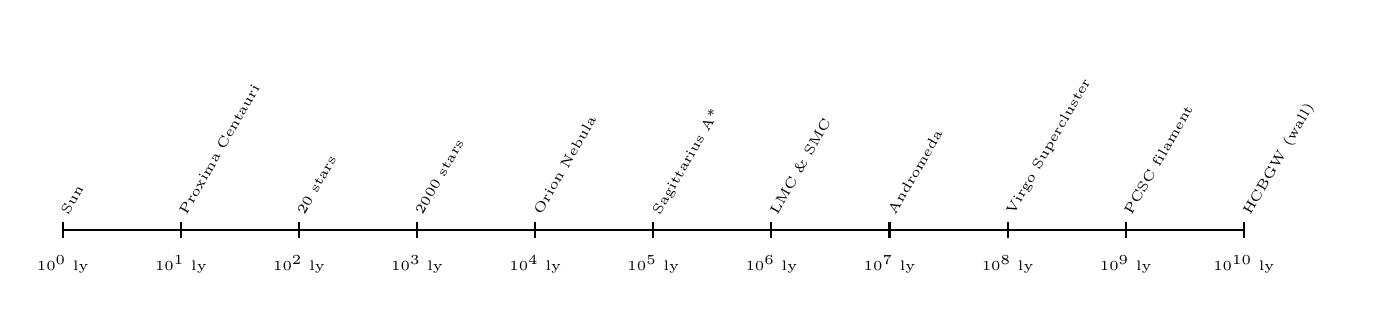
\begin{tikzpicture}
    % Parameters
    \def\n{10}
    \def\length{15}
    \def\spacing{\length/\n}

    % Labels array
    \def\labels{{"Sun", "Proxima Centauri", "20 stars", "2000 stars", "Orion Nebula", "Sagittarius A*", 
                 "LMC \& SMC", "Andromeda", "Virgo Supercluster", 
                 "PCSC filament", "HCBGW (wall)"}}

    % Draw base line
    \draw[thick] (0,0) -- (\length,0);

    % Draw tick marks, numbers and rotated labels
    \foreach \i in {0,...,10} {
        \pgfmathsetmacro{\x}{\i*\spacing}
        \draw[thick] (\x,0.1) -- (\x,-0.1); % Tick
        \node[below, font=\tiny] at (\x, -0.2) {$10^{\i}$ ly};      % Number
        
        % Multi-line labels with a 2-line approach for long labels
        \node[above, font=\tiny, text width=2.5cm, rotate=60, anchor=north west] at (\x-0.2,+0.2) 
            {\pgfmathparse{\labels[\i]}\pgfmathresult}; % Label
    }
\end{tikzpicture}
\caption{Cosmic distances span from nearby stars to the largest known structures in the universe, measured on scales of light-years, typically up to the order of 10. Each label represents either the distance to a notable astronomical object or the size of a vast cosmic region. The diameter of the observable universe is roughly 93 billion light-years, which is nearly the order of 11.}
\end{center}
\end{figure}



\subsubsection*{Milky Way in Presepective}
 
To gain perspective on the size of the Universe, it is useful to compare distances across different scales. For instance, the nearest star to the Sun is Proxima Centauri, located approximately 4.24 light-years away.  By definition, one light-year is the distance that light travels in a vacuum over the course of one year, equivalent to approximately 9.46 trillion kilometers. Within a 10 light-year radius of the Sun, there are about 20 stars, and nearly 2,000 stars lie within 100 light-years. The stars of the Orion Belt are situated at distances ranging from 800 to 1,300 light-years.

The Milky Way Galaxy is characterized by three major spiral arms—Perseus, Scutum-Centaurus, and Sagittarius—and three minor arms: the Orion Spur, Carina-Sagittarius, and Norma Arms. Our Solar System is located within the Orion Spur, a region containing millions of stars, situated between the Perseus Arm on the inner side and the Scutum-Centaurus Arm on the outer side.

\begin{figure}[htbp]
  \centering
  % Subplot 1
  \begin{subfigure}[b]{0.35\textwidth}
    \includegraphics[width=\textwidth]{../plots/0_images/Nearby_Stars.png}
  \end{subfigure}
  \hfill
  % Subplot 2
  \begin{subfigure}[b]{0.64\textwidth}
    \includegraphics[width=\textwidth]{../plots/0_images/milky_way.png}
  \end{subfigure}

  \caption{\textit{Left:} Stars located within 15ly. \textit{Right:} A segment of the Milky Way depicting the Solar System and its neighboring nebulae located in the Orion–Cygnus Arm. The Galactic Center and other minor arms - Norma and Carina–Sagittarius - are also highlighted.}
  \label{solar_system}
\end{figure}




The Perseus and Scutum-Centaurus arms seem to converge near the ends of the Long Bar, a stellar structure that stretches roughly 15,000 light-years and extends through the Galactic center. At the galaxy's core lies Sagittarius A*, a supermassive black hole believed to be the rotating nucleus of the galaxy. It is located approximately 27,000 light-years from Earth. Collectively, these elements contribute to the Milky Way's characteristic spiral disk structure, with a prominent bulge at its center.

\subsubsection*{Galactic Halo and Galaxies around}
The Milky Way’s spiral structure spans roughly 100,000 light-years in diameter, and is surrounded by a spherical halo extending up to three times that size. This halo hosts numerous satellite galaxies. One of the most prominent and easily visible from the southern hemisphere is the Large Magellanic Cloud (LMC), the Milky Way’s largest satellite galaxy, located about 160,000 light-years (50 kpc) away. The LMC itself has a satellite—the Small Magellanic Cloud (SMC)—located approximately 200,000 light-years (60 kpc) from Earth. In total, the Milky Way has over 50 known satellite galaxies. Its nearest large galactic neighbor is the Andromeda Galaxy (M31), situated around 2.54 million light-years (778 kpc) away. Andromeda is roughly two to three times larger than the Milky Way.


\begin{figure}[htbp]
  \centering
  % Subplot 1
  \begin{subfigure}[b]{0.36\textwidth}
    \includegraphics[trim= 0pt 0pt 0pt 45pt, clip, width=\textwidth]{../plots/0_images/Milky_Way_side_view.png}
  \end{subfigure}
  \hfill
  % Subplot 2
  \begin{subfigure}[b]{0.63\textwidth}
    \includegraphics[width=\textwidth]{../plots/0_images/local_group.png}
  \end{subfigure}

  \caption{\textit{Left:} Side view of the Milky Way, depicting its components and satellite galaxies, notably the Large and Small Magellanic Clouds (LMC and SMC). \textit{Right:} Spatial distribution of galaxies within the Local Group, dominated by the Milky Way and Andromeda galaxies. Source: Wikipedia - Pablo Carlos Budassi (left) and Andrew Z. Colvin (right)}
  \label{milkyway}
\end{figure}




Expanding the view to a radius of 10 million light-years, the region contains about 56 galaxies, among which the Milky Way and Andromeda are the most massive and gravitationally dominant. This collective of galaxies is known as the Local Group, which itself resides in the central region of the Virgo Supercluster.

\begin{figure}[htbp]
  \centering
  % Subplot 1
    \includegraphics[width=\textwidth]{../plots/0_images/local_superclusters.png}
  \caption{Galaxy supercluster and voids within $10^9$ ly of Virgo Supercluster. Source: Andrew Z. Colvin (Wikipedia)}
  \label{voids}
\end{figure}




\subsubsection*{Galaxy Clusters to Superclusters}
As we consider larger cosmic scales, the megaparsec (Mpc) becomes a more convenient unit for measuring distances. One megaparsec is approximately 3.26 million light-years. The Virgo Supercluster, which includes the Local Group, the Virgo Cluster, and several other galaxy clusters, spans a diameter of about 33 Mpc (roughly 100 million light-years).


The Virgo Supercluster is situated within the Laniakea Supercluster, a much larger structure that encompasses a volume about five times greater and contains approximately 100,000 galaxies. Other major regions within Laniakea include the Pavo-Indus Supercluster, the Southern Supercluster, and the Hydra-Centaurus Supercluster.

At the heart of Laniakea, within the Hydra-Centaurus Supercluster, lies a region of maximum gravitational attraction known as the Great Attractor. Most galaxies within Laniakea—including the Milky Way—are being gravitationally drawn toward this region.

\subsubsection*{Cosmic Web: Filaments, Walls and Voids}
The Laniakea Supercluster, along with the Shapley, Hercules, Coma, and Perseus–Pisces Superclusters, are all part of a vast galactic filament known as the Pisces–Cetus Supercluster Complex (PCSC). This structure is estimated to be approximately 1 billion light-years long and 150 million light-years wide, making it one of the largest known structures in the observable Universe.

Adjacent to it lies an even slightly larger filament known as the Perseus–Pegasus Filament. However, the largest known galaxy filament is the Hercules–Corona Borealis Great Wall (HCBGW), which stretches up to 10 billion light-years in length—roughly one-tenth the diameter of the observable Universe. Billions of such galaxy filaments, interwoven with gigantic cosmic voids, form the cosmic web—a vast, interconnected structure that defines the large-scale architecture of the Universe. This grand-scale pattern of matter distribution is illustrated in Figure \ref{scal}.  


\begin{figure}[htbp]
	\includegraphics[width=\textwidth]{../plots/0_images/scales}
	\caption{Large-scale structure of the Universe illustrating the cosmic web. \textit{Source: S. Stapelberg, Structures blog from the University of Heidelberg}}\label{large_scale}
\end{figure}





\section{Historical Background and Development}
Advancements in observational technology have enabled the exploration of the Universe at unprecedented depths and resolutions. These technological developments have profoundly influenced our understanding, offering novel perspectives on the evolutionary history and large-scale structure of the cosmos. This section presents a concise overview of the historical progression of astronomical research, with particular emphasis on pivotal discoveries and theoretical developments made over the past century that have fundamentally shaped contemporary cosmology.

\subsection{Distance Determination beyond the Galaxy, 1920s}
Prior to the twentieth century, the Milky Way (MW) was widely regarded as the entirety of the Universe, believed to be approximately 1.8 billion years old. The Sun was thought to occupy the central position in the cosmos, while other galaxies were misidentified as localized gaseous clouds within the Milky Way, and were classified as \textit{spiral nebulae}. This fundamental misunderstanding regarding the scale of the Universe led to a protracted debate among astronomers, most notably the Shapley–Curtis Debate in 1920, between Harlow Shapley and Heber Curtis.

A key issue underlying this debate was the inability to accurately determine the distances to these spiral nebulae. The breakthrough came with the discovery of the period–luminosity relation for pulsating stars—specifically, Cepheid variables—by Henrietta Swan Leavitt in 1912 \citep{1908leavitt,1912leavitt}. Her empirical relation, expressed as $m_{max} \propto log P$, enabled astronomers to estimate extragalactic distances with far greater accuracy. This development proved instrumental in resolving the scale of the Universe and is illustrated in Figure \ref{Leavitt-Hubble}.

\begin{figure}[ht!]
	\centering
	\begin{subfigure}[t]{0.45\textwidth}
         \centering
         \includegraphics[width=0.75\textwidth]{../plots/0_images/1912_Leavitt}
	 \label{Leavitt}
     \end{subfigure}
	\hfill
     \begin{subfigure}[t]{0.49\textwidth}
         \centering
         \includegraphics[width=\textwidth]{../plots/0_images/1929_Hubble}
	     \label{Hubble}
     \end{subfigure}
	\caption{Two remarkable discoveries of early twentieth century: a) Leavitt Law: Period (in logarithmic scale) of 25 Cepheids (of Small Magellanic Cloud) correlated with their maximum and minimum brightness. \cite{1912leavitt} b) Hubble Law: Increasing recession velocity of galaxies with respect to distance suggesting an expanding Universe. \cite{1929hubble}}\label{Leavitt_Hubble}
\end{figure}




\begin{notebox}[sharp corners, width=\textwidth]{Knowledge of Distance is fundamental in astronomy.}
Distance enables us to convert the sky’s seemingly two-dimensional projection into a three-dimensional representation of the Universe. Once the distance to a bright object is known, its true luminosity can be determined, allowing us to infer its size, mass, age and other physical characteristics.
\end{notebox}




\subsection{Expansion of the Universe}
In 1923, using the most advanced instrument of his time, the 100 - inch (2.5 m) Hooker Telescope, Edwin Hubble observed the Andromeda \textit{spiral nebula} (M31) and successfully resolved a Cepheid variable star within it. By applying the Leavitt Law (period–luminosity relation) \citep{1925hubble}, he estimated the distance to M31 and demonstrated that it lay far outside the boundaries of the Milky Way. This discovery effectively resolved the "Great Debate" in favor of Heber Curtis, confirming that Andromeda is a separate galaxy, and that the Milky Way is just one of billions of galaxies in the Universe.

Continuing his observations of Cepheid variables, Hubble measured distances to additional galaxies and identified a key relationship: the recessional velocity of a galaxy increases with its distance from the observer, expressed as $v \propto D$ \citep{1929hubble}; see Figure \ref{Leavitt-Hubble}. This empirical relation, now known as Hubble’s Law, led to the revolutionary conclusion that the Universe is expanding in all directions - a concept that contradicted Einstein’s earlier static model of the Universe \citep{1917einstein}. The constant of proportionality in this relation, known as the Hubble constant $H_0$, is of great cosmological importance, as it provides a measure of the expansion rate and thus the age of the Universe.

\subsection{The Big Bang Model, 1930s}
In the meantime, building upon Einstein’s theory of general relativity, Georges Lemaître independently arrived at the conclusion of an expanding Universe, and proposed that its earliest state was an immensely hot and dense origin \citep{1931lemaitre}. Further theoretical advances were made in 1948, when Alpher and Herman \citep{1948alpher} refined Gamow’s model of the early Universe \citep{1948gamow} and predicted the existence of cosmic microwave background (CMB) radiation—a thermal remnant of the Big Bang - at a temperature of approximately 5K.

This prediction was confirmed in 1965, when Arno Penzias and Robert Wilson detected microwave radiation with a temperature of 3.4 $\pm$ 1K using the Holmdel Horn antenna \citep{1965penzias}. Their discovery provided strong empirical support for the Big Bang model, which today stands as the standard cosmological model, describing the origin, evolution, and large-scale structure of the Universe.

\subsection{Composition of Stars}
Parallel advancements in quantum physics during the early twentieth century significantly enhanced our understanding of stellar evolution. In 1917, Arthur Eddington proposed a thermodynamic model based on free radial oscillations to explain the pulsations observed in Cepheid variable stars \citep{1917eddington}. Building on this framework, he hypothesized in 1920 that the primary source of stellar energy is hydrogen fusion into helium \citep{1920eddington}—a revolutionary idea at the time.

Further insights emerged from the study of stellar spectra. In her 1925 Ph.D. dissertation, Cecilia Payne (later Payne-Gaposchkin) demonstrated that hydrogen and helium are the most abundant elements in stars, contradicting the prevailing view that stars had compositions similar to Earth \citep{1925payne}. Her groundbreaking work established these two elements as the principal constituents of stellar matter. A comprehensive theoretical account of nuclear fusion reactions within stars was later formulated by Hans Bethe in 1939 \citep{1939bethe}, laying the foundation for modern stellar nucleosynthesis theory. It was a major leap in astronomy, as the physics of internal mechanics of stars was not well known priory, including the right mechanism behind the cyclic pulsation of Cepheid variable. 

\subsection{Age of the Universe, 1950s}
Studying stellar pulsations, Walter Baade discovered that Cepheid variables are divided into two distinct populations: Type I (classical Cepheids), which are brighter, and Type II (W Virginis stars). His recalibration of the Cepheid distance scale led to a doubling of the estimated distance to the Andromeda Galaxy and a corresponding revision of the Universe’s age from 1.8 billion to 3.6 billion years \citep{1958baade}. This estimate was further refined by his student, Allan Sandage, who extended Leavitt’s relation into a period–color–luminosity law and revised the Hubble constant to 75 km/s/Mpc in 1958 \citep{1958sandage}, resulting in an updated estimate of the age of the Universe at approximately 14 billion years. Allan's estimation lies near to modern value of Hubble constant.


\subsection{Technological Development, 1960s}
Despite numerous unresolved questions and theoretical challenges, technological advancements have significantly propelled research in astronomy, leading to major breakthroughs and providing deeper insights into the nature and evolution of the Universe. Beginning in the 1960s, the introduction of digital imaging in photometry revolutionized observational astronomy. The replacement of photographic plates with charge-coupled device (CCD) cameras markedly improved the accuracy, sensitivity, and precision of photometric measurements.

The deployment of space-based telescopes enabled observations across the entire electromagnetic spectrum, overcoming the limitations imposed by Earth’s atmosphere on ground-based instruments. Additionally, the detection of cosmic rays, neutrinos, and gravitational waves opened new avenues for studying celestial phenomena through multiple independent messengers, thereby giving rise to the field of \textit{multimessenger astronomy}. Concurrently, advances in high-energy particle physics uncovered the quantum-scale substructure of matter, contributing to more refined and physically grounded models of astrophysical processes. Collectively, these technological and theoretical developments have brought a paradigm shift in our understanding of the cosmos, marking the onset of what is often referred to as the golden era of modern astronomy.

\subsection{Composition of Universe}
Given the vastness of the universe, it is natural to wonder what it is made of. A simplified answer might be that it consists of energy and spacetime. However, energy manifests in several distinct forms undergoing different physical processes and laws. It can be heat, mass, radiation or of any other form. 

\begin{wrapfigure}{r}{0.45\textwidth}
	\begin{center}
		%\vspace{-1cm}
		\includegraphics[width=7cm]{../plots/0_images/uni_compo}
		\vspace{-1mm}
		\caption{The fractional composition of the Universe consists of dark energy (68 \%), dark matter (27 \%), and baryonic matter (5 \%) is depicted, with the contributions from radiation and other relativistic particles neglected.}
		\label{uni_composition}
		\vspace{-1cm}
	\end{center}
\end{wrapfigure}


In cosmological terms, ordinary matter, referred to as \textit{baryonic matter}, comprises electrons, protons, and neutrons, and constitutes only about 5\% of the total energy content of the universe. This baryonic matter forms the stars, galaxies, and large-scale structures we observe today. In addition to baryonic matter, dark matter represents another critical component of the cosmos. Dark matter is hypothesized to possess fundamentally distinct properties from ordinary matter, as it neither emits nor absorbs electromagnetic radiation, rendering it invisible. Its presence is inferred solely through its gravitational effects. Dark matter accounts for approximately 27\% of the universe's total energy content. Strong observational evidence for dark matter emerges from phenomena such as gravitational lensing, the anomalous rotation curves of galaxies, and the fine-scale anisotropies in the Cosmic Microwave Background (CMB). These observations, however, rely heavily on accurate distance measurements. For instance, the interpretation of gravitational lensing patterns and galaxy rotation curves depends critically on the precise determination of the distances to the lensed or orbiting objects. Despite its discernible gravitational influence, the precise nature and composition of dark matter remain unresolved, rendering it one of the most significant unsolved problems in contemporary astrophysics.

On cosmological scales, observational data further indicates that the universe is expanding at an accelerating rate, a phenomenon attributed to a hypothetical form of energy known as dark energy. Like dark matter, the exact nature of dark energy is still unknown, but it is postulated to comprise approximately 68\% of the total energy density of the universe. In stark contrast, other components, such as radiation, neutrinos, and various exotic non-baryonic particles, collectively account for less than 1\%. The study of the distribution and evolution of these components remains a vibrant and evolving field of inquiry in modern cosmology.

The determination of the relative proportions of these matter and energy components hinges on precise distance measurements across cosmic scales, as these distances are pivotal in estimating both the observed brightness and redshift of distant objects—crucial factors in reconstructing the universe’s overall composition.


\subsubsection{$\Lambda$CDM Cosmological Model}

By integrating observational data with the initial conditions established by Big Bang cosmology, scientists have formulated a standard cosmological model known as the $\Lambda$CDM (Lambda Cold Dark Matter) model. This model is defined by key parameters, including the densities of dark energy, dark matter, and baryonic matter; the Hubble constant ($H_0$); the scalar spectral index (which describes primordial density fluctuations); and the curvature parameter (which determines the geometry of the universe). Many of these parameters are tightly constrained using cosmic microwave background (CMB) measurements and are supported by various independent astronomical observations.

Accurate knowledge of cosmic distances is essential for estimating these parameters. The expansion rate, for instance, is inferred from the relationship between redshift and distance (the Hubble Law), while the discovery of the universe's acceleration was made possible by analyzing the luminosity of distant Type Ia supernovae.

Despite their differences in physical nature, the topics above share a common goal: the determination of distances to astronomical objects in order to accurately derive other physical parameters, such as size, mass, and age. Building on this idea, the primary focus of my master’s thesis is to explore distance determination methodologies, with a particular emphasis on the Leavitt Law, and to improve its accuracy by identifying and addressing sources of systematic errors. With final remarks on results implication, the last chapter concludes this thesis. 

The color gradient angular map of the sky shown in the introduction page is a snapshot of the early Universe, captured by the Planck satellite, a mission commissioned by the European Space Agency (ESA) and operational from 2009 to 2013. This map represents the Cosmic Microwave Background (CMB) radiation, which is the faint afterglow of the Big Bang. The temperature fluctuations across the sky observed in the CMB are the remnants of small density variations in the very early Universe. Over billions of years, these minute fluctuations grew due to gravitational attraction, eventually forming the large-scale structures of the Universe, including galaxies and galaxy clusters that we observe today.

The CMB is the most ancient relic we can witness from the early Universe, offering a direct glimpse into the conditions that prevailed just 380,000 years after the Big Bang. These observations allow scientists to infer important properties of the Universe's early state, such as its age, composition, and rate of expansion. One of the most significant results derived from the Planck data is the precise determination of the Hubble constant ($H_0$), which quantifies the current rate of expansion of the Universe. The value of $H_0$ is crucial for understanding the Universe's past and predicting its future evolution. 

When observing the Universe at great depths, we are essentially looking into the past, as light takes time to travel through space. This fundamental property allows us to study the early Universe and its evolution. One method of measuring the expansion rate of the Universe involves determining the distance to the farthest observable objects—essentially, measuring the distance to the cosmological horizon, the farthest point from which light has had time to reach us since the Big Bang.

To validate the Hubble constant ($H_0$) obtained from local measurements, we use a method known as the cosmic distance ladder. This method involves calibrating several different distance measurement techniques, each suitable for different scales of the Universe. These methods begin with relatively nearby objects and work outward to increasingly distant galaxies, eventually reaching the cosmological scale, where measurements can be compared to the results obtained from the Planck mission and other independent methods. By calibrating each step of the distance ladder, we can achieve a more accurate and consistent measure of cosmic distances, which in turn helps refine our understanding of the expansion rate of the Universe.

However, recent studies have revealed a discrepancy in the measured values of the Hubble constant, especially when comparing results from local measurements (such as Cepheid variable stars and the Tip of the Red Giant Branch method) to those obtained from the cosmic microwave background (CMB) observations, like those from the Planck mission. This discrepancy has come to be known as the $5-\sigma$ Hubble Tension. It refers to a statistical difference at the 5-sigma level, indicating a significant mismatch between the two methods. This tension has sparked a great deal of debate in the cosmological community, leading to numerous investigations into potential new physics that might explain the difference.


\subsection{Cosmic Distance Ladder and Hubble Constant}

One of the most pressing issues in modern cosmology is the growing discrepancy in the measured value of the Hubble constant ($H_0$)—the rate of expansion of the universe. Early-universe measurements, primarily derived from observations of the Cosmic Microwave Background (CMB) using the Planck satellite and interpreted within the $\Lambda$CDM cosmological model, yield a value for $H_0$ that significantly differs from those obtained via direct measurements in the local universe \citep{2018planck, 2021freedman}. This tension, now known as the \textit{Hubble tension}, challenges our understanding of cosmology and may point to new physics or systematic errors yet to be uncovered.

Late-universe estimates of $H_0$ are derived by correlating redshifts with distances of astronomical objects. Because no single method spans the full range of cosmic distances, astronomers rely on a sequence of interconnected techniques known as the \textit{cosmic distance ladder}. Each “rung” of the ladder is calibrated by more fundamental, closer-range methods to extend reliable distance measurements farther into the universe.


\begin{wrapfigure}{r}{0.45\textwidth}
	\begin{center}
		\vspace{-1cm}
		\includegraphics[width=7cm]{../plots/0_images/ladder}
		\vspace{-1mm}
		\caption{An instance of Cosmic Distance Ladder calibrating Leavitt Law with parallax, SNIa with Leavitt Law and Hubble Law with SNIa based distances. \citep{2022riess}}
		\label{ladder}
		\vspace{-1cm}
	\end{center}
\end{wrapfigure}




A key breakthrough in refining the distance ladder came from Adam Riess and collaborators, who studied Type Ia supernovae (SNIa) in distant galaxies. These explosive events, originating from white dwarf mergers, follow a predictable relation between their intrinsic brightness and the width of their light curves. By calibrating SNIa with Cepheid variable stars via the Leavitt Law, Riess extended high-precision distance measurements from the local 30 Mpc range ($\sim 10^8$ ly, Cepheid-based) to beyond 1000 Mpc ($ \sim 10^{10}$ ly) using SNIa as \textit{standard candles}—objects with known intrinsic luminosity \citep{1998riess}.

Figure~\ref{ladder} illustrates the cosmic distance ladder, starting from geometric parallax for nearby stars, advancing through Cepheid variables, and culminating in SNIa-based distances for high-redshift galaxies. Using this refined framework and fitting distances to the Hubble law derived:

\[
H_0 = 73.30 \pm 1.04 \; \text{km s}^{-1} \text{Mpc}^{-1}
\]
a result in $5\sigma$ tension with the Planck-inferred value under $\Lambda$CDM assumptions \citep{2022riess}. Resolving this discrepancy remains a top priority in cosmology, potentially revealing insights into dark energy, new particles, or modifications to the standard model of the universe.


\subsection{Golden Era of Astronomy - Gaia onwards}
The launch of the Gaia satellite by the European Space Agency (ESA) in 2013 marked a significant leap in modern astronomy. Utilizing the geometric parallax method with the baseline of Earth’s orbital diameter, Gaia has precisely measured the distances to over 1.8 billion stars within the Milky Way and its surrounding regions, while simultaneously conducting extensive photometric and astrometric observations of the sky. The exceptional accuracy of Gaia's measurements has established a new standard for distance calibration in astronomical research. This research work relies on distance measurements obtained from the parallax data of Gaia Data Release 3 (DR3). 

In 2021, the launch of the James Webb Space Telescope (JWST) by NASA further advanced the observational capabilities. With its sensitivity to the far-infrared spectrum, JWST has begun to reveal unprecedented details of the early Universe, including the formation of the first galaxies and stars. In addition to these missions, a number of major cosmological surveys and observatories—such as SDSS, Planck, and 2dFGRS—have already made transformative contributions to our understanding of the cosmos. Looking ahead, the commissioning of next-generation facilities, including the Vera C. Rubin Observatory, DESI, 4MOST, Euclid, SKA, and LISA, is expected to redefine the frontiers of observational astronomy and cosmology, setting new benchmarks for future research.


\section{Scope of this Thesis}


\begin{wrapfigure}{r}{0.4\textwidth}
	\begin{center}
		\vspace{-1.2cm}
		\includegraphics[width=6cm]{../plots/0_images/Storm2011.png}
		\vspace{0mm}
		\caption{\textit{K-band Period-Luminosity relation for Galactic Cepheid using IRSB distance.} Source: Storm J., 2011}\label{PLjesper}
		\vspace{-1cm}
	\end{center}
\end{wrapfigure}


The aim of this thesis is to improve the accuracy of Galactic Leavitt Law - a primary distance indicator of cosmic distance ladder. Note the large scatter in linear period-luminosity relation of Cepheids, giving uncertainity to the slope and zero point of the fit. Using such a period-luminosity relation as a reference for the next rung of distance scale leads to larger error in the measurements, making it crucial to have a tight PL relation in the first place - to gain a high confidence on the cosmological scale studies. To refine the Leavitt Law to its finest form, I will be taking following steps which will be briefly discussed in following chapters. 

\begin{itemize}
\item Identify and omit the outliers from BVIJHK photometric dataset of Galactic Cepheid.
\item Estimate intrinsic luminosity of observed targets using reddening and Gaia DR3 parallax. 
\item Determine error in distances and interstellar reddenings following the method of \cite{2017madore}.
\item Reformulate the Leavitt Law with distance-reddening corrected intrinsic luminosity of Cepheids.
\item Cross validate the calibrated Leavitt Law with Cluster Cepheid based Leavitt Law.
\item Apply the refined Leavitt Law on LMC and SMC Cepheids to determine their distances.
\end{itemize}

\subsection{Part I: Parameters of Leavitt Law}
The period-luminosity scatter plot requires primarily two parameters of Cepheid variables: a) accurate measurement of pulsation period, and b) accurate estimation of intrinsic luminosity of the respective Cepheid star. The Figure \ref{PLjesper} depicts an instance of Leavitt Law in K band, where distances to invidual stars measured by infrared surface brightness (IRSB) method \citep{2011storm}, and interstellar extinction derived using Fouque's extinction law \citep{2007fouque} and Fernie's reddening measurements \citep{1994fernie}. 

The pulsation periods of Cepheid variables are determined from light curves based on photometric observations spanning multiple pulsation cycles. This parameter is well-constrained for all Cepheid targets considered in this study. The primary focus of this research, however, lies in determining the second essential quantity—the intrinsic (absolute) luminosity of these stars. While telescopes measure the apparent luminosity, estimating the absolute luminosity requires correcting for both the distance the light has traveled and the attenuation caused by interstellar extinction.

Stellar light is subject to scattering and absorption as it traverses the interstellar medium, particularly through dust and gas clouds along the line of sight. Any imprecision in correcting for these effects leads to significant deviations from the expected linear relationship in the period-luminosity relation. Consequently, accurately quantifying the uncertainties in distance and interstellar reddening for each Cepheid is a central objective of this thesis.

The first part of this thesis is dedicated to a detailed examination of these parameters and their interdependencies, as outlined in the next chapters.

\subsection{Part II: Calibration Method and Dataset}
This part of thesis contains three chapters covering details on Galactic Cepheid dataset, calibration methodology, its related physics and comparision plots. The Galactic Cepheid dataset used in this thesis contains multiband photometric data in the BVIJHK bands. The extinction law developed by Cardelli et al. \citep{1989cardelli}, in combination with the total-to-selective extinction ratio adopted from Sandage \citep{2004sandage}, is employed to convert the color excess values compiled by Fernie into BVIJHK extinction. Using parallactic distance estimates from the Gaia mission and extinction, raw Leavitt Law are derived. 

The calibration technique used in this thesis is devised by Barry Madore \citep{2017madore}. Utilizing the reddening-free nature of the Wesenheit function \citep{1982madore}, the effect of reddening and distance errors on individual Cepheid can be decoupled and traced by comparing the residuals of BVIJHK period-luminosity relation with residual of period-wesehiet relation. In his paper, Madore had used V -  I based  wesenheit function to determine the errors and ultimately tighten the multiband PL relations. In this thesis, first, I applied the same method on B -  V, V -  K and J -  K based wesenheit functions, and compared the deviation in resulting distance-reddening error-pair for individual star, for each color index case. Secondly, I modified the methodology from generic wesenheit function to composite wesenheit function and repeated the exercise to derive the error-pairs for individual Cepheid for each color indicies. It lead to some crucial insights about wesenheit function and its dependency on the reddening ratio and color index. Finally, the calibrated Leavitt Law cross-validated with an additional dataset of 18 Galactic cluster Cepheids - more reliable distance measured by averaging parallax of the cluster members hosting the Cepheids. 

This part of the thesis ends with a discussion on the results. 

\subsection{Part III: Result Implications}

\subsubsection*{LMC \& SMC Distance}
To test the effectiveness, LMC and SMC distances have been derived for 24 versions of calibrated Leavitt Law, i.e. 6 photometric bands with 4 colors of wesenheit functions. With such multiple possibilities, a distance matrix can be made highlighting effectiveness of particular color index used in calibration, with respect to the rest.

In astronomy, distance is not just a measurement - it's the foundation upon which our understanding of the universe is built. From determining the true luminosity of celestial bodies to constraining the age, scale, and rate of expansion of the cosmos, accurate distance measurements are indispensable. The physical interpretation of almost every astronomical observation - be it the brightness of a star, the motion of a galaxy, or the composition of the universe - depends critically on knowing how far away the object lies. Throughout this section, we will see how the knowledge of distance informs our understanding of cosmic composition, the expansion rate, or the evolution of the Universe. 



\part{Parameters of Leavitt Law}
%
\chapter{Observables - Luminosity, Reddening, Distance}


% Apply a background image to the epigraph region
\begin{tikzpicture}[remember picture, overlay]
  % Place the image (background) in the epigraph area
  \node[anchor=north west, opacity=0.5, scale=1.1,yshift=4cm,xshift=-0.2cm] at (current page.north west) {
    \includegraphics[width=\paperwidth]{../plots/0_images/nebula.png} % Your image path
  };
\end{tikzpicture}



%\epigraph{Who really knows? \\ Who will unfold it? \\ How did this Universe formed?\\ Where does it come from? \\ Gods came after the creation. \\ Then, who really witnessed the origin of this existence?} {Rigved X.129.6}


%https://science.nasa.gov/asset/webb/cosmic-cliffs-in-the-carina-nebula-nircam-image/


\section{Why does a star shine?}
The Sun, a luminous and intensely hot star, derives its fundamental properties from the enormous gravitational forces acting within its structure. Possessing a mass approximately 333,000 times that of Earth, the Sun’s vast mass is confined within a relatively compact volume, resulting in a continuous gravitational contraction toward its core. This inward collapse generates extremely high pressures and densities, particularly in the central regions. Consequently, core temperatures rise to several million Kelvin, establishing the conditions necessary for nuclear fusion to occur. Within this high-energy environment, surpassing the Coulumb barrier protons collide and fuse to form heavier atomic nuclei, predominantly helium.

At the core of the Sun, approximately 700 million metric tons of hydrogen are converted into helium each second through fusion processes, liberating a tremendous amount of energy. A substantial fraction of this energy is carried away by neutrinos, with a minor portion possibly emitted as gravitational waves. The remainder propagates outward as electromagnetic radiation, manifesting primarily as heat and visible light. This radiant energy escapes the solar surface and travels through space as sunlight, a fraction of which reaches Earth. Upon entering Earth's atmosphere, solar radiation interacts with atmospheric molecules, undergoing scattering that redistributes the light. The portion of the electromagnetic spectrum that penetrates the atmosphere - referred to as the optical band - corresponds to the visible range and is perceived as the bright solar illumination observed from Earth.

\textit{The total energy emitted by the Sun across all wavelengths per unit time is defined as its luminosity}.  

As this radiation traverses the Earth's atmosphere, part of it is absorbed or scattered, a process collectively termed atmospheric extinction. This mechanism modulates both the intensity and spectral distribution of solar radiation at the Earth’s surface. A similar attenuation of starlight occurs in interstellar space, known as \textit{interstellar extinction}, wherein light is absorbed or scattered by interstellar dust and gas. This process affects the transmission of radiation between stellar sources rather than through a planetary atmosphere.

A notable consequence of extinction is the wavelength-dependent nature of absorption and scattering, a phenomenon known as \textit{reddening}. Because shorter wavelengths (i.e., blue light) are more efficiently scattered than longer wavelengths (i.e., red light), light passing through such media often exhibits a shift toward redder colors. This reddening effect serves as a crucial diagnostic tool in astrophysics, enabling the characterization of the intervening interstellar medium and enhancing our understanding of the distribution and composition of cosmic dust and gas.

\section{Light: Color and Luminosity}
Light is a form of electromagnetic (EM) radiation that travels through space at a constant speed of 299,792,458 meters per second in a vacuum. The human visual system is sensitive to a narrow portion of this spectrum, known as the optical band, which ranges from approximately 350 to 700 nanometers wavelength. This segment represents only a small fraction of the full electromagnetic spectrum, which spans from high-energy gamma rays to low-energy radio waves.

The electromagnetic spectrum also describes the distribution of thermal radiation emitted by objects at various temperatures. When matter is heated, it emits energy in the form of electromagnetic radiation. As the temperature increases, the peak of this emission shifts toward shorter wavelengths and higher frequencies, corresponding to a greater energy output. This fundamental relationship between temperature and spectral energy distribution (SED) is described by Planck’s law \citep{1900planck}, which provides the theoretical foundation for the modern understanding of blackbody radiation and underpins much of contemporary astrophysics.



\begin{wrapfigure}{r}{0.4\textwidth}
	\vspace{-0.5cm}
	\includegraphics[width=\linewidth]{../plots/0_images/Blackbody_spectra}
	\caption{\textit{Black body radiation curves based on Planck’s Law for various temperatures. The maxima of the curves shift according to Wien’s displacement law.  Source: Wikipedia commons}}
	\label{blackbody}
	\vspace{0.3cm}
\end{wrapfigure}



According to Plank law, a perfect black body absorbs all the incident radiation and emits radiation across the entire electromagnetic spectrum. His formulation of spectral energy distribution as a function of wavelength is given as: 

\begin{equation}
	B_\lambda (T) = \frac{8 \pi h c}{\lambda^5 (e^{\frac{h c }{\lambda k T }} - 1)}
\end{equation}

where $B_\lambda$ is radiant energy at given wavelength in [$W.m^{-2}.sr^{-1}.m^{-1}$] unit, $\lambda$ is wavelength, $h$ is Planck's constant, $k$ is Boltzmann constant, $c$ is speed of light and T is the temperature of the object. Integrating it for all the wavelength yields the total energy output of the blackbody at given temperature.  

To estimate radiation flux emitted towards the observer, integrating $B_\lambda (T)$ over the hemisphere above the emitting surface:
\begin{equation}
	F_\lambda(T)= \int B_\lambda(T) cos \theta d \omega = \pi B_\lambda(T)
\end{equation}


Now, consider a star of radius $R$ that emits a spectral radiation flux $F_\lambda$ at temperature T. At a distance $d$ from the star, the flux measured by a detector is governed by the inverse-square law, which states that the observed flux decreases with the square of the distance from the source. Accordingly, the observed flux $f_\lambda$ at distance $d$ is given by:

\begin{equation}
f_\lambda = {\frac{R}{d}}^2 F_\lambda
\end{equation}

If the sensitivity of detector given by sensitivity function, $E_\lambda$, the total radiation flux recieved by the detector would be

\begin{equation}
s= \int_{0}^{\infty} f_\lambda E_\lambda d \lambda
\end{equation}

The amount of flux recieved by a detector measured as photon count per wavelength range, called as \textit{band}, which further converted into more convinient unit of measurement called as \textit{magnitude}. It is the standard unit of measurement of light in photometry. 

\subsection{Magnitude Scale}
Ancient Greek astronomer, Hipparchus  (c. 190 – c. 120 BCE), had made a star catalogue						 by defining a scale of brightness for stars in the units of magnitude (mag), where '1 mag' refers to the brightest and 6 mag is the dimmest star in the sky, for unaided eye. The definition of magnitude scale revisited by V.Pogson in 1850 and calibrated by J.F. Zöllner in 1861 by using visual photometer. They made a comparison in between an artificial star and a real star using two Nicol prisms to redefine a precise magnitude scale. 

According to Pogson's definition, difference between 'apparent magnitudes' of two stars is proportional to the logarithmic of their radiation flux ratio ($s_1/s_2$). i.e.

\begin{equation}
m_1 - m_2 = 2.5 \log(s_1/s_2)
\end{equation}
It follows as if the magnitude of two stars differ by 5, that means one star appears 100 times brighter than the other star. For instance, it is measured that $\alpha$  Lyr (Vega) has visual magnitude of 0.14 mag and $\alpha $ Cyg (Deneb) has 1.33 magnitude which is fainter than $\alpha$ Lyr. Sun, Moon, Venus, Mars, Jupiter and three stars - Sirius, Canopus and $\alpha$ Centauri are the only celestial objects having negative apparent magnitude, count among the brightest objects in the night sky. 


\subsection{Color Index \textit{($m_1$ - $m_2$)}}
The visible band of light is a small window of electromagnetic spectrum corresponds to the wavelength ranging from 300 nm (Blue) to 700nm (Red). The difference in the photon intensity at different wavelength
translated as different color index. If one observes the night sky carefully, it would be clear that stars come in different colors, and their magnitude differs on observing with different color bands. For instance, if one observes the sky in red band, Betelguse would appear brighter than Sirius, even if Sirius is the brightest star. It is because Sirius emits its most of the radiation in blue band, while betelguse radiates in red band. It is due to their photosphere's temparature differences.

To determine the precise stellar colors and magnitudes, W.W. Morgan and H. L. Johnson developed UBV system of color bands with effective wavelenght for ultraviolet$_\lambda: 365$ nm , blue$_\lambda: 440$ nm, visual$_\lambda: 548$ nm ) \citep{1953johnson}. Further extension of the UBV system into the red and infrared passband was done by adding following filters in [$\mu m$].
$$
\begin{array}{cccccccccc}
Bands & R & I & J & H & K & L & M & N & Q\\
\lambda_{eff} & 0.7 & 0.9 & 1.25 & 1.63 & 2.2 & 3.6 & 5.0 & 10.6 & 21
\end{array}
$$

\subsubsection*{Temperature \textit{$(T_{eff})$}}

While studying stellar spectra, K. Schwarzchild recognised that the color incides measures the energy distribution, thus it could be used to estimate the temperature of photosphere of the star. 

On fitting energy distribution with Plank radiation law, in Wien's approximation ($c_2/(\lambda T) >> 1$), the radiation flux results
\begin{equation}
F_\lambda \propto exp(-c_2/(\lambda T_c))
\end{equation}

For the sake of simplicity, let the sensitivity function of the photo-detector be at its maxima, then the relation in between color index, B - V , and the effective temperature of the star would be.

\begin{equation}
B - V = \frac{2.5 c_2 \log e}{T_C} \left(\frac{1}{\lambda_B} - \frac{1}{\lambda_V} \right) + const.
\end{equation}

with radiation constant $c_2 = 0.014 mK$, $\lambda_B = 440 nm$ and $\lambda_V = 548nm$,

\begin{equation}
B-V = \frac{0.7 * 10^4}{T_c} + const.
\end{equation}

The above equation suggests that the color indices (B-V) corresponds to temperature of the star. 



Refering $\alpha$ Lyr (Vega - A0V type star) as a standard star, the magnitude scale, in U, V and B bands, defined in such a way that : 

\begin{equation}
U-B = B-V = 0
\implies C_{UB} = C_{BV} = 0
\end{equation}

For convenience, the notation for color $U-B$ is adopted as $C_{UB}$. Color index $C_{BV}$ less than 0.5 indicates blue and more than 1.5 indicates red. 




\vspace{2cm}

\subsection{Absolute Magnitude (\textit{M})}
When a luminous object is observed from different distances, it appears to have varying brightness because flux decreases with increasing distance. So, how can we compare the intrinsic brightness of two remote stars?  To enable standardized comparisons, astronomers adopt a reference distance of 10 parsecs (pc). The radiant flux of a star measured at this distance defines its \textit{absolute magnitude}, denoted as $M_\lambda$. The subscript $\lambda$ indicates the specific photometric band (filter) used in the observation, as brightness varies across different bands.

Given this framework, if $m_\lambda$ represents the apparent magnitude of a star observed at a distance \textit{d} (in parsecs), and $M_\lambda$ is its absolute magnitude, the relationship between them is given by the following formula:

$$M_\lambda = m_\lambda - 2.5\log \left( \frac{d[pc]}{10}\right)^2 $$
\begin{align}
M_\lambda = m_\lambda - 5\log{d[pc]}  + 5 
\end{align}

The above is a simple relation which relates the observable luminosity with the distance of any stellar object. 

\begin{notebox}[sharp corners, width=\textwidth]{True Absolute Magnitude}
The above relation must be corrected for the effect of interstellar extinction, $A_\lambda$, to obtain the correct \textit{'photometric'} distance. 
\begin{align}
M_\lambda^0 = m_\lambda - A_\lambda - 5\log{d[pc]}  + 5 
\end{align}
\end{notebox}


\section{Distance}
The introductory chapter makes it clear that the standard units of length used in everyday life are inadequate for astronomical measurements. To address this, astronomers have developed a distinct set of units for measuring astronomical distances. However, different units are used depending on the spatial scale. For example, within the solar system, the astronomical unit (AU) is sufficient, while on the scale of the Milky Way, the light-year is more appropriate. For even larger distances, such as those in extragalactic realm, units like the parsec or megaparsec are commonly used. The relationships between these units are summarized in Table 

\ref{table:distance}.
\begin{table}[h!]
	\centering
	\caption{Conversion of Astronomical Distance Units}
	\begin{tabular}{c |c c c c} 
		
		 & Kilometer & Astronomical Unit & Light Year & Parsec\\  
		\hline
		Kilometer & 1 &  &  &\\ 
		Astronomical Unit & 149597870.700 & 1 &  &\\
		Light Year & 9460730472580.8 &  63241.077 & 1 &\\
		Parsec & 30856775814913673 & 206264.806247096 &  3.261563777 & 1\\ 

	\end{tabular}
	\label{table:distance}
\end{table}

\subsection{Parallax: Measuring Astronomical Distances Using Geometry}

Parallax is a geometrical method that utilizes trigonometric principles to measure the distance to an object by observing its apparent shift relative to a fixed background, caused by the movement of the observer. While measuring distances between nearby objects on Earth is straightforward using tools like rulers or laser rangefinders, this becomes impractical when dealing with vast astronomical distances. Hence, astronomers rely on methods such as parallax, Leavitt Law, etc.

The choice of method for measuring astronomical distances depends on both the scale of the measurement and the characteristics of the celestial object in question. Since no single technique is effective across all distance ranges in the universe, astronomers must understand the physics of various astrophysical phenomena in order to select the most appropriate method for a given situation. Accurate distance measurement is foundational in astronomy, as it affects our understanding of everything from stellar properties to the large-scale structure of the cosmos.

One of the fundamental tools used in determining distances is trigonometry. In a right-angled triangle, if one side and an angle (other than the right angle) are known, the other sides can be calculated using trigonometric ratios. There are six basic trigonometric functions: sine (sin), cosine (cos), and tangent (tan), along with their respective reciprocals: cosecant (csc), secant (sec), and cotangent (cot). These ratios depend solely on the angle and not on the actual size of the triangle, making them highly useful in astronomical applications where distances are vast and direct measurement is impractical.

\begin{wrapfigure}{r}{0.35\textwidth}
	\begin{center}
		\vspace{-10pt}
		\includegraphics[width=5cm]{../plots/0_images/parallax}	
		\caption{ As Earth orbits the Sun, nearby stars appear to shift against distant background stars—this shift, called parallax, is used to measure their distance using trignometric ratio. \tiny \hfill \textit{Source: hyperphysics.phy-astr.gsu.edu}}
		\label{parallax}
	\end{center}
\end{wrapfigure}






In the context of stellar parallax, a conceptual triangle is formed between the Earth, the Sun, and a distant star. The baseline of this triangle is the distance between the Earth and the Sun, known as 1 Astronomical Unit (AU). As Earth moves in its orbit over the course of six months, nearby stars appear to shift slightly against the backdrop of more distant stars. This apparent angular shift is called the parallax angle. Because the triangle formed is extremely elongated, the parallax angle is very small, typically measured in arcseconds.

To calculate the distance to a star using the parallax method, astronomers apply the tangent trigonometric ratio, which in this context is:

\begin{equation}
\tan p = \frac{1 AU}{d}
\end{equation}

For very small angles (as in astronomical observations), $\tan p$ is approximately equal to $p$ when measured in radians. Therefore, the distance can be simplified to:

\begin{equation}
d = \lim_{p \to 0} \frac{1 AU}{\tan p} = \frac{1 AU}{p} 
\end{equation}


To standardize distance measurements, astronomers use the parsec as a unit of length.

\vspace{0.3cm}
\begin{center}
\textit{1 parsec (pc) is defined as the distance at which 1 AU subtends an angle of 1 arcsecond (1/3600 of a degree).}
\end{center}
\vspace{0.3cm}

The Gaia satellite, launched by the European Space Agency in 2014, has revolutionized our understanding of the Milky Way by measuring the parallax and proper motion of billions of celestial objects. Among the vast number of objects observed, several notable types of variable stars, including Cepheid variables and RR Lyrae stars, were also studied. In this thesis, the parallax-driven distances provided by Gaia will be used to calibrate the period-luminosity relation. 

\subsection{Distance Modulus ($\mu$)}

A useful parameter for denoting distance in astronomy is the distance modulus, $\mu$, which provides a logarithmic transformation of the distance to an object, using 10 parsecs as the reference distance. The distance modulus can also be expressed as the difference between the apparent magnitude and the absolute magnitude of an object. Mathematically, it is formulated as:

$$\mu = m - M = 5 log_{10}\left[\frac{d}{10 pc}\right] $$ 
 


\section{Interstellar Reddening}

In photometric observations, the electromagnetic flux of starlight is quantified by counting the incoming photons within a specific wavelength range of the spectrum. Intervening gas in interstellar space absorbs most of the high-energy photons (X-rays and extreme ultraviolet, EUV) and scatters much of the light in the B and V bands. Radiation with wavelengths longer than the size of dust particles can pass through the interstellar medium largely unaffected, making the sky nearly transparent to infrared, microwave, and radio waves. The diminishing of short-wavelength luminosity makes the source appear redder than its intrinsic color, giving rise to the effect known as reddening.



\begin{wrapfigure}{r}{0.45\textwidth}
	\vspace{-0.4cm}
	\centering
	\includegraphics[width=\linewidth]{../plots/0_images/extinction}
	\caption{ \small{Comparision between emitted (0) and observed (1) SEDs. For given band, deviation between the curves represents interstellar extinction (here, $A_B$ and $A_V$). On the right side, the relative difference between extinction of two bands depicting the definition of interstellar reddening $E(B-V)$. \citep{1993krelowski}}}\label{extinction} 
	\vspace{-0.7cm}
\end{wrapfigure}





This phenomenon can be illustrated by comparing the observed SED of stellar light to the theoretical SED predicted by Planck's Law, as shown in Figure \ref{extinction}. \\
Let B and V be the apparent luminosities of a star as received by the observer, while $B_0$ and $V_0$ represent the intrinsic (unextincted) luminosities. Then, the effect of extinction can be formulated as follows:
\begin{align}
A_B = B - B_0 \\
A_V = V - V_0 
\end{align} 

The difference between the two defines the \textit{color excess} - that is, the deviation of a star's apparent color from its intrinsic color. 
\begin{align}
E(B-V) = A_B - A_V = (B - V) - (B - V)_0 
\end{align} 

Color excess is more widely used than extinction to describe the effect of the ISM on starlight, as it can be measured photometrically even when the intrinsic brightness of the star is unknown. 

\subsection{Reddening Ratio}
The ratio of total-to-selective absorption, $R_\lambda$ summarizes the effect of extinction and reddening on the intensity of light along the line-of-sight. It is formulated as:

\begin{align}\label{eq:reddening_ratio}
R_\lambda^{BV} = \frac{A_\lambda}{E(B-V)}
\end{align}

For Milky Way, the reddening ratio in V-band, $R_V$, is evaluated about 3.23 \citep{2004sandage}, whereas in B-band it set to be as $R_B$ = $R_V + 1$

Rearranging the above relation and writting it as:
\begin{align}\label{eq:extinction}
	A_\lambda =& R_\lambda E_{BV} = R_\lambda (A_B - A_V) 
\end{align}
The above equation is used for transforming measured color excess into extinction for any band, provided $R_\lambda$ is priorily known.  Rearranging it further, for V-band, the equation takes the form:
\begin{align}
	\frac{A_B}{A_V} = & 1 + \frac{1}{R_V}
\end{align}

\cite{1989cardelli} generalised the extinction law in this form for all the bands with V-band as reference as discussed in the following section. 

An another important aspect of the reddening ratio is to convert color excess from one pair of bands, say $E_{BV}$ to another, $E_{1 2}$. It can be done as follows:

\begin{align*}
E_{12} = (R_{1}^{BV} - R_{2}^{BV}) E_{BV} 
\end{align*}


This leads the transformation law for reddening ratio $R_\lambda$:

\begin{align}\label{R_transform}
    R_\lambda^{12} = \frac{R_\lambda^{BV}}{R_1^{BV} - R_2^{BV}}
\end{align}

The values of $R_\lambda^{BV}$ are calculated by \cite{2007fouque} and given in Table \ref{Tab:fouque}.

\subsection{Interstellar Extinction Law}


\begin{wrapfigure}{r}{0.35\textwidth}
	\centering
	\vspace{-0.9cm}
	\includegraphics[width=\linewidth]{../plots/0_images/CCM_1989.png}
	\caption{ \small{Galactic extinction law fitted for UBRIJHKL along three directions in the sky, with varying $R_V$, with $A_V$ as reference. \citep{1989cardelli}}}\label{extinctionlaw} 
	\vspace{-0.45 cm}
\end{wrapfigure}




Observations of the spectral energy distribution (SED) of stellar light by \cite{1966Whiteoak} demonstrated the diminishing effect of interstellar extinction at longer wavelengths. This finding led to the formulation of an extinction law - an inverse relation between extinction and the wavelength of stellar light. In its simplest form, the extinction law formulated as \citep{1989cardelli}: 

\begin{align}\label{eq:CCM_1989}
	\frac{A(\lambda)}{A(V)} =& a(\lambda^{-1}) + \frac{b(\lambda^{-1})}{R_V} 
\end{align}

Here $a(\lambda^{-1})$ and $b(\lambda^{-1})$ are determined empirically for different spectral ranges. Since, historically, observational data in the V-band were available for most stars, extinction in the V-band has been used as a reference. The Figure \ref{extinction} depicts that a variation in $R_V$ leads to changes in extinction law, where short wavelength have significantly affected as compared to longer wavelengths. Using the averaged value over all the directions in the Milky Way for $R_V = 3.23$ and the formulation \eqref{eq:CCM_1989}, \cite{2007fouque} evaluated the extinction law for BVRIJHK bands as given in the Table \ref{fouque}


	\begin{table}[ht]
		\caption{Extinction Law and corresponsing reddening ratio adopted from Table 4 of \cite{2007fouque} }
		\centering
		\vspace*{3mm}
		\begin{tabular}{c c c c}
			\hline
			Band filters & Effective Wavelength  &  Extinction Law & Reddening ratio \\ 
			 & \mbox{$\lambda$ ($\mu$m)} & \small{$\frac{A(\lambda)}{A(V)} = a_{\lambda} + \frac{b_\lambda}{R_V}$} & \small{$R_\lambda = \frac{A_\lambda}{A_V} \times R_V$}\\
			\hline 
			B & 0.438 & 1.31  & 4.231\\
			V & 0.545 & 1     & 3.230\\
			I & 0.798 & 0.608 & 1.963\\
			J & 1.235 & 0.292 & 0.943\\
			H & 1.662 & 0.181 & 0.584\\
			K & 2.159 & 0.119 & 0.384\\
			\hline 
			\end{tabular}
		  \label{fouque}
	\end{table}

  




\subsection{Wesenheit Magnitude}
To account for the effects of reddening, \cite{1982madore} introduced a method based on a pseudo-magnitude derived from the reddening ratio, known as the Wesenheit magnitude. By definition, this quantity is constructed to be free from the effects of reddening. Its mathematical formulation is derived as follows:

\begin{align*}
R_\lambda^{12} & = A_\lambda / E_{12} \\
    & = \frac{m_\lambda - m_\lambda^0}{(m_1 - m_2)-(m_1 - m_2)_0} \\
\end{align*}

On rearranging the terms, 

\begin{align}
m_\lambda - R_\lambda^{12}(m_1 - m_2) & = m_\lambda^0 - R_\lambda^{12}(m_1 - m_2)_0 \\
W_\lambda^{12} & = W_0
\end{align}

It can be observed that, on the left-hand side, all terms except R are observables, while the right-hand side consists of absolute quantities. This implies that if R is known a priori with high precision, the Wesenheit magnitude will yield the same value for both reddened and unreddened sources, effectively making it a reddening-free parameter. \\


\begin{notebox}[sharp corners, width=\textwidth]{Equvivalent Wesenheit Magnitude}
For wesenheit magnitude, the following relation holds true for any color index ($m_1 - m_2$) 
\begin{align}
W_\lambda^{12} =W_0^{12} 
\end{align}
\end{notebox}




A comparison of the definitions of the 'true' absolute magnitude and the Wesenheit magnitude in relation to the color index (B-V) reveals:

\begin{align}\label{mag_eq}
    M_\lambda^0 & = m_\lambda - R_\lambda^{BV} \times E(B-V) - \mu
\end{align}

\begin{align}\label{wes_eq}
    W_\lambda^{BV} & = m_\lambda - R_\lambda^{BV}  \times (B-V) - \mu
\end{align}

It can be observed that absolute magnitude depends on four types of measurements: photometric magnitude, distance, reddening ratio and color excess. In contrast, Wesenheit magnitude requires only three types of measurements and does not depend on color excess. Let's examine how these magnitudes vary with errors in measurement. Assuming that the \textit{apparent luminosities are precisely measured ($\delta m_\lambda = 0$), the adopted extinction law is accurate  ($\delta R = 0$), implies the errors contribution divided among the distance modulus ($\delta \mu $) and color excess ($\delta E_{BV} $) measurements} in the case of an individual Cepheid. Error in above equations leads to:

\begin{align}\label{mag_error}
    \delta M_\lambda & = - ( R_\lambda^{BV}* \delta E(B-V) + \delta \mu)
\end{align}

\begin{align}\label{wesen_error}
    \delta W_\lambda^{BV} & = - \delta \mu
\end{align}

This pair of equations indicates that both the Wesenheit magnitude and the absolute magnitude are sensitive to distance errors. However, unlike the absolute magnitude, the Wesenheit magnitude remains unaffected by errors in reddening. This characteristic of the Wesenheit magnitude is particularly important, as it helps to decouple the errors contributions of distance and reddening for individual Cepheids. \\

Application of these equations in the Leavitt Law calibration will be discussed in the \textit{Part II} of this thesis. 


%\chapter{Pulsating Star - Classical Cepheid}


% Apply a background image to the epigraph region
\begin{tikzpicture}[remember picture, overlay]
  % Place the image (background) in the epigraph area
  \node[anchor=north west, opacity=0.5, scale=1.1,yshift=10cm,xshift=-0.3cm] at (current page.north west) {
    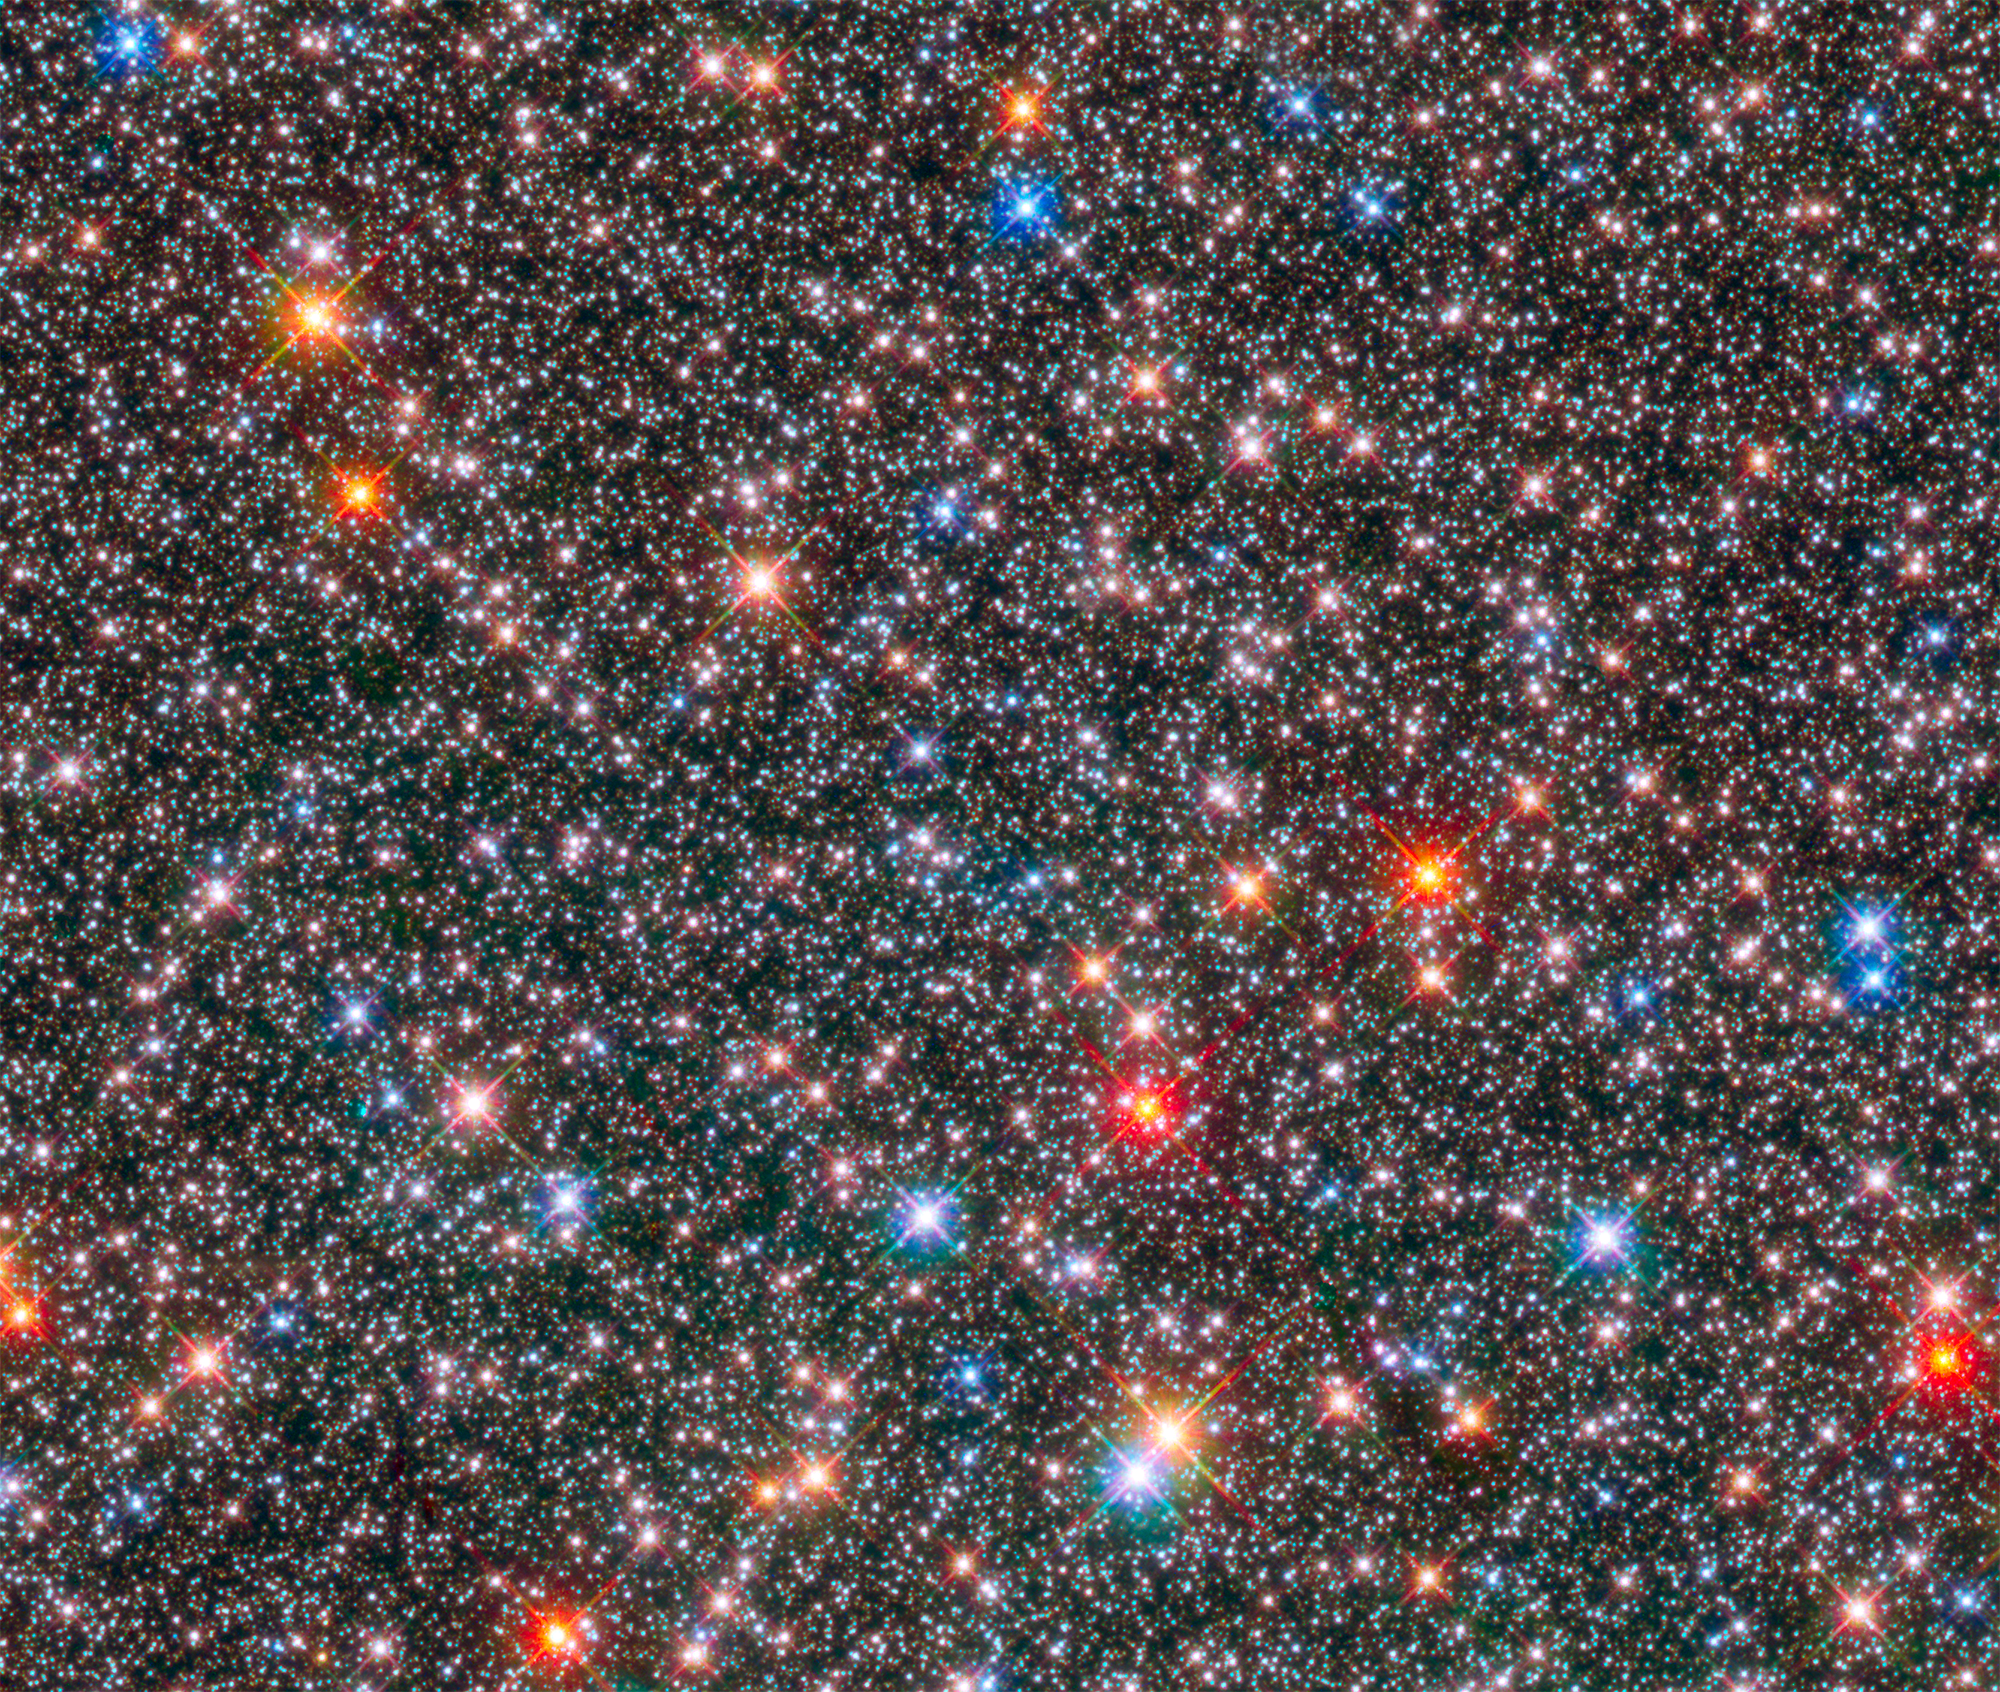
\includegraphics[width=\paperwidth]{../plots/0_images/crowd.png} % Your image path
  };
\end{tikzpicture}



%\epigraph{Who really knows? \\ Who will unfold it? \\ How did this Universe formed?\\ Where does it come from? \\ Gods came after the creation. \\ Then, who really witnessed the origin of this existence?} {Rigved X.129.6}


%https://science.nasa.gov/asset/hubble/milky-way-bulge/



\section{Are all stars the same?}
Seeing the night sky, one can easily spot that stars come in different colors and luminosities, making it easy to infer that not all stars are the same. But what makes them appear different? With the advent of quantum mechanics and spectroscopic observation, this question was answered by explaining the physical processes occurring inside the star, along with changing chemical potential over the different evolutionary phases of the stars. It has been observed that some stars can be thousands of times larger than others—such as red giants and supergiants — while some undergo radial oscillations periodically, like RR Lyrae, Cepheids, and Mira variables. Some stars may form diffuse gaseous systems, such as protostars and planetary nebulae, while others could be the remnants of dead stars, like white dwarfs or neutron stars. These examples represent different phases in the life cycle of a star. This chapter delves into these evolutionary stages, examining how astronomers classify stars, discussing their underlying physics, while focusing particularly on Cepheid variables.

\subsection{Discovery of Variable stars}
The year 1784 is significant in astronomy, as it was when John Goodricke observed the luminosity variation of a star in Cephus consellation - Delta Cephei - challenging the centuries-old belief that the sky is static i.e. all stars being fixed and unchanging \cite{1786john}. Motivated by such a remarkable discovery, the hunt for more variable stars began. Inheriting the name from the first one, variable stars of a similar class were classified as Cepheid variables. Until the twentieth century, it was unclear to astronomers why do Cepheids vary in luminosity. Some suggested a pair of eclipsing binaries \cite{1899pickering} \cite{1903myers} \cite{1914shapley} but spectra shown that it was a single star; others proposed interior effects due to stellar magnetic fields \cite{1908hale} \cite{1914russellvariables} though pulsation was not correlating with magnetic cycle of the star; and some supported the idea of tidal deformation of star's envelope \cite{jeans1917tidal} but light curve did not match with rotation of star. Contribution from Arthur Eddington played a central role in the development of the pulsation theory towards the right path. Mimicking the physics of a reversible heat engine and conceptualized through a valve mechanism (periodically blocking and releasing heat), Eddington formulated the radial pulsation theory of Cepheid variables named as $\kappa$-mechanism \cite{1917eddington}.

Modeling chemical composition and drawing inspiration from Eddington’s valve mechanism for stellar pulsations, Zhevakin, in 1953, proposed that the cyclical ionization of helium envelope drives the radial oscillations observed in Cepheid variables \citep{1963zhevakin}. He modeled a spherical shell consisting of an 85\%–15\% hydrogen–helium mixture (by number of atoms), where helium transitions between the transparent HeI and opaque HeIII states. These ionization transitions modulate the opacity of the stellar envelope, leading to variations in surface brightness and pulsation behavior in Cepheids.

Further developments by S. Chandrasekhar in the hydrodynamic and magnetohydrodynamic stability provided a foundational approach for modelling stellar interior for different masses in various phases \cite{1949chandrasekhar} \cite{1961chandrasekhar}. Utilizing hydrodynamic theory with thermal condition for the stability of Cepheid variable, Cox developed the equation of state of such radially oscillating system \cite{1959cox} . His contribution through non-adiabatic pulsation theory explained $\kappa$- mechanism in detail - how ionized Helium layers changing opacity leads to instability region in Hertzsprung-Russell diagram, also called as instability strip \cite{1968cox} \cite{1980cox}. 

Following in this chapter, a brief summary on the physics of stars and their evolution is discussed. 


\section{Stellar Evolution}
Over the course of their lifetimes, stars vary in size and luminosity depending on their evolutionary phase. Hertzsprung was the first to plot the brightness of a star cluster against its color \cite{1911hertzsprung}, revealing an underlying evolutionary trend. Soon after, Russell independently reached to the similar conclusions \cite{1914russell}. In their honor, this diagram is now called the Hertzsprung-Russell (HR) diagram. For a student of Astrophysics, understanding the color-magnitude is the first step as it play fundamental role in understanding the stellar evolution processes undergoing in different kind of stars.

Stars are classified into three broad categories based on their mass: low-mass, intermediate-mass, and massive stars. These categories follow different evolutionary tracks over their lifespan. As the accumulated matter in a region contracts gravitationally, it reaches stages of threshold densities and temperatures, where different nuclear fusion reactions occur in a natural sequence, starting with hydrogen (1 proton) and progressing to silicon (14 protons + 14 neutrons) which could ultimately fuse to form iron at extreme temperature of 3 billion K . Energy transformation from mass to radiation, heat, neutrino emission, gravitational waves, and other forms is well modeled by quantum physics and gravitational physics, ultimately leads to theory of stellar evolution. In this section, I will briefly summarize the physical processes occurring during the different phases of evolution for each category of star. Following this, we will develop an understanding of the physics behind the pulsations of Cepheid variable stars.

%\begin{figure}[h!]
	\begin{center}
		\includegraphics[width=\textwidth]{../plots/0_images/evol}
	\end{center}
	\caption{Evolutionary cycle for low and high mass star. Low mass stars, like Sun, become a Red Giant when Hydrogen supply to the core stops and fusion takes place in the shell around the core. Afterwards they become a Planetary nebula with a bright core at the center and end their life as a White Dwarf, slowly get faded turning into brown dwarf. Massive stars evolve to Red Supergiant and end their life as Supernova leaving behind either a Neutron star or Black Hole.  [cmglee/NASA Goddard Space Flight Center] }		\label{evolution}
\end{figure}

 
\begin{figure}[h!]
	\centering
	\vspace{-0cm}
	\includegraphics[width = 0.8\textwidth]{../plots/0_images/1992_chiosi}
	\caption{\cite{1992chiosi} HRD}
	\label{1992_chiosi}
\end{figure}
 

\subsection{Formation of Star}

In the vicinity of interstellar nebulae, dispersed gas can collect into dense cloud-like structures called globules, composed mostly of molecular hydrogen (H₂) with trace amounts of heavier elements. Due to the intrinsic mass of the gas, regions of sufficiently high density begin to gravitationally collapse, creating a pressure gradient that slowly raises the core temperature to around 10–30 K. Thermal motion of molecules and radiative cooling initially balance the collapse, stabilizing the temperature for a period. As the collapse continues, the density increases, leading to higher opacity, blocking the radiation causing a gradual rise in temperature. When core temperatures reach roughly 60–100 K, thermal pressure becomes significant enough to temporarily halt the collapse, forming the first hydrostatic core. According to the virial theorem, as mass continues to accumulate, the core temperature rises further.

Once the core temperature reaches approximately 2000 K, molecular hydrogen begins to dissociate, absorbing energy and slowing the temperature rise. This triggers a second, rapid collapse until the core temperature reaches ~10,000–20,000 K, at which point hydrogen becomes fully ionized. The second hydrostatic core is established, supported by the thermal pressure of dense, opaque ionized hydrogen. During this stage, the core’s rotation causes the formation of a rotating accretion disk of infalling material. Gas in the disk follows the trajectories determined by the gravitational potential, often guided along magnetic field lines. Along the polar regions, magnetic pressure dominates over gas pressure, accelerating ionized gas along open field lines and producing highly collimated, supersonic bipolar jets, which manifest observationally as Herbig–Haro objects.

At temperatures ranging from 60 to 100 K, thermal pressure halts the continous gravitational collapse As the protostar continues to accrete mass, it contracts over the Kelvin–Helmholtz timescale, converting gravitational energy into heat. The core temperature steadily rises, eventually reaching $~10^7$ K, sufficient to initiate nuclear fusion.

Nuclear fusion requires that atomic nuclei come sufficiently close for the strong nuclear force to bind them together. However, the positive charges of the nuclei cause Coulomb repulsion, forming the Coulomb barrier. Only at the extreme temperatures and pressures in the protostar’s core do nuclei achieve enough kinetic energy to overcome this barrier. When hydrogen nuclei fuse, primarily via the proton–proton chain, four hydrogen nuclei combine to form one helium nucleus, releasing energy as photons and neutrinos. The onset of sustained hydrogen fusion marks the birth of a star, which enters the main-sequence phase of stellar evolution.

\input{chapters/content/0_3_plot_1934_bethe.tex} 

The first fundamental nuclear reaction in stellar cores is the formation of deuterium (a nucleus containing one proton and one neutron), which occurs at core temperatures of approximately 10–18 million Kelvin. In this process, two protons (hydrogen nuclei) collide at very high velocities, sufficient to overcome the Coulomb barrier and approach within the range of the strong nuclear force (on the order of femtometers). To stabilize the newly forming nucleus, one of the protons undergoes a β⁺ decay (positron emission) process, in which a proton converts into a neutron. At the quark level, this corresponds to an up quark (charge +2/3 e) changing into a down quark (charge –1/3 e), accompanied by the emission of a positron (e⁺) and an electron antineutrino (ν̅ₑ). The resulting proton and neutron then bind together via the strong nuclear force to form a deuterium nucleus. This reaction is the first step in the proton–proton chain, a series of nuclear reactions that release a tremendous amount of energy. The energy output generates radiation pressure, which counteracts the inward pull of gravity, stabilizing the protostar and sustaining its roughly spherical structure over thousands to millions of years.

The first basic nuclear reaction, the formation of Deuterium (nucleus containing one proton and one neutron), requires a temperature of 10 - 18 million Kelvin. In this senario, two protoniums (hydrogen ions) collide with each other at a very high velocity, surpassing the Coulomb barrier and entering to field of strong nuclear force at femto scale. To stablise the new configuration, one of the proton changes its up quark (+1/3) to down quark (-2/3), releasing positron and an electron antineutrino, to converts into a neutron. This process is called as $\beta^{+}$ decay process. Both elementary particles, proton and neutron, stick together to form nucleus of Deuturium. Series of such nuclear reactions release an immense amount of energy radiating outwards. Radiation pressure counter balances the continous gravitation collapse of the matter, sustaining the spherical structure of the protostar for thousand to million years. The energy released from fusion reactions in stars calculated by Bethe and published under title - 'Energy production in stars'\citep{1939bethe}. At the heart of these calculation, Einstein's famous equality $E = \Delta m c^2$ underlies which tranforms mass into energy. Here, c is the speed of light and $\Delta m$ is the difference between the mass of reactants and products of the fusion reactions. 


\begin{notebox}[sharp corners, width=\textwidth]{Nuclear Fusion Reactions in Main Sequence Star}

{\small Accumulation of Deuterium opens possibility for fusing with one more proton to form Helion (2 protons and 1 neutron). Rising temperature fuses two Helion atoms to form Helium (2 protons and 2 neutrons) and emits two Hydrogen atoms. This series of reactions from Hydrogen to Helium is called p-p chain (pp I branch) reaction. Other rarer reactions can also occur, for instance, pp II branch when Helion fuses with Helium to form Beryllium (4 protons and 3 neutrons). Then either Beryllium decays to Lithium (3 protons and 4 neutron), Lithium fuses with proton and breakdown into two Helium atoms. Otherwise, in pp III branch, Beryllium fuses with proton to form Boron (4 proton and 4 neuton) which is unstable and breaks down into two Helium. The most rare case is pp IV branch, when Helion captures a proton and form Helium. 
%Source: F. Reines, Ann. Rev. Nucl. Sci. 10 (1960) 1-26}
}

Proton-Proton Reactions: Efficient for 1 $M_0$ star's core. \\

\hspace{1cm} Branch I: 83.30\% Helium production, at 10-18 MK


\begin{center}
	\ce{^1H ->[p][e+,$\nu_e$]^2D ->[^1H][ $\gamma$ ]  ^3He ->[^3He][2 ^1^H] ^4He } 	
\end{center}
%\vspace{-3mm}

\hspace{5.6cm} 0.42 \hspace{0.7cm} 5.49 \hspace{0.7cm} 12.85  \hfill (Energy release in MeV)

\hspace{1cm} Branch II: 16.70 \% Helium production, at 18-25 MK

\begin{center}
	\ce{^4He ->[He][$\gamma$]^7Be ->[e-][ $\nu_e$]  ^7Li ->[H] 2 ^4He }	
\end{center}
\vspace{-2mm}
	\hspace{5.6cm} 1.59 \hspace{0.6cm} 0.861 \hspace{0.3cm} 17.35 \hspace{0.9cm} \hfill (Energy release in MeV)
	\vspace{1mm}

\hspace{1cm} Branch III: 0.12\% Helium production, above 25 MK

\begin{center}
	\ce{^4He ->[He][$\gamma$]^7Be ->[H][ $\gamma$]  ^8B ->[][e+,$\nu$_e] ^8Be -> 2^4He }	
\end{center}
\vspace{-2mm}
	\hspace{4.9cm} 1.59 \hspace{0.6cm} 5.59 \hspace{1.7cm}     23.29   \hfill (Energy release in MeV)


\hspace{1cm} Branch IV: 0.00002\% Helium generation in Sun 

\begin{center}
	\ce{^3He ->[H][e+,$\nu$_e] ^4He}	
\end{center}
	\hspace{7.1cm} 19.795 \hspace{0.3cm}  \hfill (Energy release in MeV)
	
{ \small All these four branches are called pp chain reaction.}
\end{notebox}


The fusion of elements releases vast amounts of heat, radiation and neutrino flux. A star's evolution depends primarily on its initial mass. Massive stars experience stronger gravitational pressure, higher core temperatures, and faster fusion rates, causing them to burn through their fuel more quickly and live shorter lives compared to lower-mass stars. Stars progress through several phases during their evolution, driven by their mass, as shown in Figure \ref{evolution}.


\vspace{1cm}


\subsection{Main sequence star and Turn-off point}



The color of the star gives a rough idea about the surface temperature as well as evolutionary phase of the star. Newly born stars are rich in Hydrogen and fuse it rigorously resulting very high surface temperature making it appear bluer. After millions of years, helium as byproduct accumulates at the core which blocks the supply of Hydrogen and reduces the rate of fusion due to which star cools down and turn yellowish. It is worth to say that, high mass stars exert high pressure at core and burn its fuel quickly as compare to low mass stars. Where lifespan of a high mass star (8-10 $M_\odot$ ) lies around 10-15 million years, for low mass star it can be 15-20 billion years. In its life journey, any star spends most of the time in Main Sequence phase.

\begin{wrapfigure}{r}{0.4\textwidth}
	\centering
	\vspace{-0.7cm}
	% include first image
	\includegraphics[width=\linewidth]{../plots/0_images/Evo2.png}  
	\label{isochrone}
	%\begin{center}
	\caption{Isochrones of stars with different masses depicting their evolutionary traids.  Source: Universe (VIII edition) by Roger A. Freedman \& William J. Kaufmann III}
\end{wrapfigure} 




For the case, when the initial mass of star remained under half of solar mass, after a few billion years, enough Helium get depleted at the core which blocks the hydrogen supply, ultimately reducing the rate of fusion reaction. Star gets cooler with time, finally become redder then a brown dwarf and its life as a black dwarf after trillions of year. Such star never leaves the main sequence but only changes its spectral type as it evolves. For star of one solar mass, when Helium core forms which reduces the rate of fusion reaction, the gravitation pull begins to contract the core and core's temperature increases again. With higher temperature, Hydrogen begins to fuse around the Helium core in a shell, making the star move away from the main sequence and marks the turn-off point in the HR diagram. 

\subsection{Red Giant Star and Helium Flash}
Shell burning Hydrogen generates even more energy than core burning phases. Released energy pushes the envelope of matter outwards which expands the surface of the star enormously and it becomes a giant. With increased surface area and shell H-burning, luminosity of the star increases by the order 3 to 4, however, due to expansion, surface of the star cools down making it red in color. This physical characteristics gives it name - Red Giant. Further accumulation of Helium at the core due to H-shell burning continuous. Star having mass more than 3 solar mass, gradually star helium burning at the core, however stars with mass between 0.3 to 3 solar mass attain Helium fusion spontaneously, called as Helium Flash. For the latter case, central region of the core becomes incompressible but the rest of core still collapses causing further rise in temperature at center, but not sufficiently enough that helium could fuse, so the central core takes the form of degenerate matter to balance the gravitation collapse. 

Around 300 million K, the degenerate matter spontaneously fuses into heavier elements, Carbon and Oxygen, by triple alpha process leaving behind a flash of high energy which rises the temperature exponentially high. Degenerate matter fuses rapidly rising the temperature even higher which accelerate the reaction rate. This thermal runaway reaction increases the energy production of the star to 100 billion times for a very short time, which is comparable to entire galaxy's energy output. Eventually thermal pressure becomes dominant and the core expands. This phase in HR diagram can be observed as the tip of the red gaint branch on the right-upper side for intermidiate mass (0.4 to 3 solar mass). Just after this state, star rearranges its structure rapidly and attain an equilibrium state with a lower luminosity but higher temperature than before. This spontaneous process shifts the star from red gaint branch to horizontal branch while leaving a discontnuity in between the two regions in HR diagram. \footnote{Kristen. B. W. McQuinn et al 2019 ApJ 880 63}    

\subsection{Horizontal branch and Variable stars}

While evolving through horizontal branch, stars fuse Helium at the core and Hydrogen in a shell. Moving towards right side, star enters to the blue edge of instability strip of HR diagram where it experience a dynamic equilibrium between gravitational contraction of outer envelope and its thermal expansion due to energy generation from internal processes. This translated as a radial oscillatory motion of the surface, giving birth to a new category of stars called variable stars. In 1784, John Goodricke had discovered a variable star, $\delta$ Cephei, in Cepheus constellation and named the star as $\delta$ Cephei. After the discovery of a few more variable stars, the family of $\delta$ Cephei type stars called as Cepheid stars. 

Initially, it was assumed that the periodic variation of luminosity arising because the star is a member of eclipsing binary system. In 1917, Arthur Eddington rejected the prior theory and gave a clever explanation behind the radial pulsation of star by purposing a valve mechanism. His purposed mechanism known as Kappa mechanism as kappa stand for coefficient of absorption of stellar material. After excessive burn of hydrogen, helium becomes the next abundant element on the surface. Due to high temperature at the compressed state of Cepheid star, Helium releases its both electrons and get ionized \ce{He^{2+}}. Opaque \ce{He^{2+}} blocks the outcoming radiation making the star appear dimmer. The radiant energy develops a pressure and expands the star's surface. The expansion increases the surface area illuminating the star. Expansion also cools down the surface so the ionized Helium captures the free electrons and back to its ground state \ce{He}. Neutral Helium is a transparent gas consequently, all the trapped radiation releases making the star even more luminous. As the radiation pressure decreases, the stellar surface begin to collapse again due to gravitational pull and shrinks down to original state. This brings the process to its initial state.   

\subsection{AGB Stars and Planetary Nebulae}
In a time scale of 100 million years, star evolve through the instability strip and exits from red edge of the instability strip towards right in HR diagram. At this stage, Helium fusion process continues in a shell around the Carbon/Oxygen core making star luminous then Red Giant phase and even bigger in size, comparable to the orbit of the Earth. In HR diagram, it moves alongside the Red Giant branch which gives it name Asymptotic Giant Branch. After Helium shell runs out of fuel, outer layer of Hydrogen burning becomes the dominant source of energy and produces Helium. After 100 thousand years, Helium accumulates and ignites again spontaneously which expands the outer surface of the star even more. Expansion cools down the temperature which halts the Hydrogen shell burning. In the next hundreds of years, Helium burning stops and Hydrogen burning take place to produce more Helium. This cycle of energy production in shells along with Helium shell flash processes expel 50\% to 70\% of star's mass in the interstellar space, bringing AGB stars to its end as a planetary nebula. The radius of planetary nebula can reach upto 30 light years (nearest star to the Sun, Proxima Centauri is about 4.2 lightyears away). 

\input{chapters/content/0_3_plot_stellar_evolution.tex}



\subsection{Super Novae and Compact Objects}
After fusing Helium and Hydrogen in shell, Carbon and Oxygen rich core forms at the center. By passing through AGB and then planetary nebula phase, star release its most of mass as stellar wind and the core remains as the remnant of dead star, countering the gravitational collapse by electron degneracy pressure as there is not active nuclear fusion going on. Such an object is called White Dwarf. S. Chandrasekhar, in 1930s, developed a theory about such compact object and purposed that such object can not exceed its mass more than 1.44 times of solar mass. This number is known as Chandrasekhar limit. 

As per the initial mass of the star, it could reach to three end points of its life - a) White dwarf, b) Neutron star or c) Black Hole. White dwarf is the remnant of a dead star whose core is mainly composed of degenerate matter. At this stage, there is no active nuclear fusion process going inside white dwarfs as there is not enough mass remaining to rise the core temperature for further fusion process. To sustain the system, the electron degeneracy pressure balances the gravitational collapse in White Dwarfs. 

If a white dwarf exceeds its mass than 1.44 solar mass, then gravitational pull dominates the electron degeneracy pressure and spontaneous thermal runaway reaction initiates the fusion process of carbon to heavier elements like neon, oxygen, magnesium, silicon, sulfur, argon, calcium, titanium, chromium, iron to nickel. This process emits an immense amount of energy and the event is called as Type Ia Super Nova, where Ia is the luminosity class. There are other types of super novae (or novae) also occur from different range of masses of stars, however, Type Ia SNe are set as standard candle with absolute luminosity of -19 mag approx. Formation of Neutron star and Black hole results from more massive stars compare to the progenitor of white dwarfs. 



\section{Pulsation of Cepheid}

More classical studies done long ago by
Cox, King, and Tabor (1973) show that the
Cepheids will not pulsate unless the helium
content is at least Y=0.25 \cite{1973cox}

\begin{wrapfigure}{r}{0.5\textwidth}
	\centering
	\vspace{-0cm}
	\includegraphics[width = 0.6\textwidth]{../plots/0_images/1926_eddington}
	\caption{\small \cite{1926eddington} Chapter Eight of The internal constitution of the stars.}
	\label{1926_eddington}
\end{wrapfigure}


\begin{wrapfigure}{r}{0.5\textwidth}
	\centering
	\vspace{-0cm}
	\includegraphics[width = 0.6\textwidth]{../plots/0_images/1926_binary}
	\caption{\small \cite{1926eddington} abandoning eclipsing binary theory.}
	\label{1926_binary}
\end{wrapfigure}


\begin{figure}[h!]
	\centering
	\vspace{-0cm}
	\includegraphics[width = \textwidth]{../plots/0_images/1968_pulsation}
	\caption{\small \cite{1968pulsation} Understanding pulsation mechanism in fourty years}
	\label{1968_pulsation}
\end{figure}


\textit{If the leakage of heat decreases during compression and increases during expansion, then driving of pulsation is possible.} \cite{1998noels}

\subsection{Light Curve}
In 1926, while analysing the light curve of Cepheid variable, Hertzsprung noticed a systematic trend in the shapes of light curve with respect to period which is called Hertzsprung progression.
\cite{1981Simon} He noticed that the Cepheids with period less than 6 days has nearly sinusodial light curve and as the period increases to 10 days, a bump appears on the descending part of light curve which progesses towards maximum light and crosses the maximum light for Cepheid of period greater than 10 days.  

\subsection{Kappa Mechanism}

The kappa mechanism is a key process that drives the pulsations in Cepheid stars. 

It operates within the outer layers of the star, specifically in the partially ionized regions where the opacity, represented by the Greek letter kappa ($\kappa$), changes significantly with temperature.

The pulsations in Cepheids are characterized by radial expansion and contraction of the outer layers, causing the star to periodically brighten and dim. 

The kappa mechanism is responsible for triggering these pulsations by influencing the balance between gravity and radiation pressure in the star's interior.

    Opacity and Temperature Sensitivity: Opacity refers to the ability of a medium to absorb and scatter radiation. In Cepheid stars, the opacity is affected by the degree of ionization within the outer layers. At certain temperatures, the opacity experiences a sharp increase, leading to a localized region called the opacity bump.

Expansion and Contraction: During the pulsation cycle, the outer layers of the Cepheid star expand during maximum brightness and contract during minimum brightness. As the star expands, it cools down due to the decrease in temperature. Conversely, during contraction, the temperature increases.

Partial Ionization: As the star expands, the temperature decreases in the outer layers, causing some previously ionized atoms to recombine with electrons, resulting in partial ionization. This ionization state is crucial for the kappa mechanism to operate effectively.

Opacity Bump Effect: Within the partially ionized regions of the Cepheid star, the temperature reaches a point where the opacity is relatively high. This increased opacity affects the balance between gravity and radiation pressure. When the opacity is high, the radiation pressure becomes less effective at counteracting gravity, causing the outer layers to contract.

Energy Transfer: The contraction of the outer layers increases the temperature, reducing the degree of ionization. As a result, the opacity decreases, allowing the radiation pressure to become more efficient. This increased radiation pressure then pushes against gravity, causing the outer layers to expand.

Feedback Loop: The expansion of the outer layers leads to a decrease in temperature, triggering recombination and an increase in opacity. This increased opacity restricts radiation pressure, causing the outer layers to contract again. This cycle repeats, creating the pulsations observed in Cepheid stars.

\section{Hydrogen Ionization Front:}
At base of HIF, opacity increases sharply limiting the depth of Cepheids photosphere. Hydrogen ionizes at 6000K \cite{1995kanbur}

Motion HIF over envolopes \cite{1971keller}


\section{Leavitt Law}

To obtain the total luminosity LL of a star (total power emitted across all wavelengths and directions), you integrate over the star's entire surface area and over all wavelengths:


\begin{align}
	L= & \int_{0}^{\infty} (4 \pi R^2 F_\lambda(T)) d \lambda \\
	 = & 4 \pi^2 R^2 \int_{0}^{\infty} B_\lambda(T) d \lambda \\
	 = & 4 \pi R^2 \sigma T^4
\end{align}



On plotting a scatter plot in between period and luminosity,a linear relation in between both the parameters  with a certain scatter 


The period-luminosity relation (also known as the Leavitt Law or the Cepheid period-luminosity relation) is an empirical relationship that exists between the pulsation period and the intrinsic luminosity of Cepheid variable stars. This relationship allows astronomers to determine the distance to Cepheids and calibrate the cosmic distance ladder.

The period-luminosity relation was first discovered by American astronomer Henrietta Leavitt in the early 20th century while studying the brightness variations of Cepheid stars in the Small Magellanic Cloud. Leavitt found that there was a consistent relationship between the periods and the average luminosities of these stars.

The period-luminosity relation states that the longer the period of a Cepheid star's pulsation, the more luminous it is. In other words, there is a direct correlation between the pulsation period and the intrinsic brightness of the star. This relationship allows astronomers to use the observed period of a Cepheid star to determine its intrinsic luminosity.

Once the intrinsic luminosity is known, the apparent brightness (or magnitude) of the star can be measured. By comparing the intrinsic luminosity with the apparent brightness, astronomers can calculate the distance to the Cepheid star using the inverse square law of light.

The period-luminosity relation is valuable because it provides a reliable and relatively straightforward method for determining distances to Cepheids and, subsequently, to other celestial objects. By measuring the period of a Cepheid star's pulsation, astronomers can estimate its intrinsic luminosity, and from that, they can determine its distance by comparing it to the observed brightness.

The period-luminosity relation has been refined over the years through extensive observations and analysis of Cepheid stars in various galaxies. It has become an essential tool for measuring cosmic distances and has played a vital role in our understanding of the scale of the universe, the expansion rate of the universe (Hubble's Law), and the calibration of other distance indicators, such as Type Ia supernovae.




\part{Calibration Method and Dataset}
\input{chapters/4_Dataset.tex}
\input{chapters/5_Calibration.tex}
%\part{Result Implications}
%\chapter{Discussion}

\section{Reddening Comparison}
\cite{2009ApJ...696.1498M}


\section{Distance Comparison}

\section{Luminosity Comparison}

\begin{figure}[h]
	\centering
	\includegraphics[width=\linewidth]{M_V}
\end{figure}

\section{Effect of Metallicity}

\cite{2009MNRAS.396.1287S}
%\chapter{Conclusion}

\section{Result}


\section{Application Of The Result}

%\part*{Appendix}
%\chapter*{Appendix}

\section*{Mathematical Tools}

\subsection*{Linear Regression}
sdas
\section*{Baade-wesselink method}



%line{toc}{chapter}{Appendix}
\bibliographystyle{apalike}
\addcontentsline{toc}{chapter}{Bibliography}
\bibliography{references}
\end{document}

